\documentclass[11pt,a4paper]{article}
% Generated from research/paper/manuscript/supporting_information.md by research/paper/analysis/md2tex.py (no pandoc); not compiled in the authoring environment.
\usepackage[utf8]{inputenc}
\usepackage[T1]{fontenc}
\usepackage{lmodern}
\usepackage{textcomp}
\usepackage{amsmath,amssymb}
\usepackage{graphicx}
\usepackage{booktabs,longtable,array,pdflscape,tabularx}
\usepackage[margin=2.3cm]{geometry}
\usepackage[numbers,sort&compress]{natbib}
\usepackage{xcolor}
\usepackage{hyperref}
\hypersetup{colorlinks=true,linkcolor=blue!50!black,citecolor=blue!50!black,urlcolor=blue!50!black}
\setlength{\tabcolsep}{3pt}
\setlength{\emergencystretch}{3em}
\title{Supporting Information --- QCM frequency and dissipation estimation using DDS excitation, gain--phase detection and complex-admittance reconstruction}
\author{openQCM NEXT impedance-analysis working group\thanks{Author list and affiliations to be finalised.}}
\date{Draft v0.2 --- 2026-10-08}
\begin{document}
\maketitle

\noindent\emph{Every number in this document is regenerated from the raw data by the scripts in \texttt{research/paper/analysis/} (\texttt{run\_estimators.py}, \texttt{run\_glucose.py}, \texttt{run\_v2.py}, \texttt{run\_bias\_theory.py}, \texttt{run\_forward\_model.py}, \texttt{make\_figures\_v2.py}, \texttt{make\_si.py}); the tables below are written by \texttt{make\_si.py} from \texttt{results/v2/asis/*.csv}. Variant "as acquired" unless stated; the firmware-corrected variant is in \texttt{results/v2/fwfix/} and Section S7.}

\section{Literature comparison, full table}

The full comparison table (hardware architecture, sweep method, measured quantities, phase measured, complex $Y/Z$ reconstructed, BVD fitting, Lorentzian fitting, frequency estimator, dissipation estimator, liquid validation, multi-overtone, real-time suitability, computational complexity, cost class), with the verification grade of each entry, is \texttt{research/paper/literature/comparison\_table.md}; the literature review and the novelty assessment are \texttt{literature\_review.md} and \texttt{novelty\_assessment.md} in the same folder. The compact Table 1 of the main text is its first block.

\section{Small-load approximation to Kanazawa--Gordon: sources and checks}

The derivation of main-text Eqs. (1)--(4) was carried out twice independently (\texttt{notes/derivations.md} §6 and \texttt{notes/theory\_sla\_to\_kg\_check.md}). The points verified against the sources: (i) the SLA normalises the complex shift to the \emph{fundamental} $f_F$ and is applied at the overtone frequency $f_n = nf_F$ inside the load impedance, which is what produces $\Delta f_n \propto \sqrt n$ \citep{Johannsmann2008, Johannsmann2021}; (ii) with $\exp(i\omega t)$ the imaginary part of the shift is $+\Delta\Gamma$ and the Newtonian impedance is $(1+i)\sqrt{\omega\rho\eta/2}$, so $\Delta\Gamma_n = -\Delta f_n > 0$; (iii) for $n = 1$ Eq. (4) is the relation of Kanazawa and Gordon \citep{KanazawaGordon1985AC}. Numerical check with $\rho_q = 2648$ kg m$^{-3}$, $\mu_q = 2.947\times10^{10}$ Pa ($Z_q = 8.83\times10^6$ kg m$^{-2}$ s$^{-1}$), $f_F$ = 5 004 596 Hz (DS-2) and 5 000 107 Hz (DS-3): coefficient 715.04 and 714.08 Hz per $\sqrt n$ per unit $\sqrt{\rho\eta}$; water ($\sqrt{\rho\eta}$ = 0.9420 kg m$^{-2}$ s$^{-1/2}$, NIST Chemistry WebBook, IAPWS-95 density and IAPWS 2008 viscosity \citep{NISTWebBookWater}) 673.6 and 672.7 Hz$\cdot$$\sqrt n$; isopropanol (1.2616, handbook values 781.0 kg m$^{-3}$ and 2.038 mPa s; Kerscher et al. \citep{Kerscher2024} measure 780.9 and 2.07) 902.1 Hz$\cdot$$\sqrt n$ (910 Hz with Kerscher's values). The 2021 tutorial writes the SLA as its Eq. (23) with $f_0$ the fundamental and derives its Eq. (29), $(-1+i)\sqrt n\sqrt{f_0}\sqrt{\rho\eta}/(\sqrt\pi Z_q)$, for the Newtonian liquid, which is Eq. (4) of the main text; the 2008 and 1985 primary texts were not reachable from this session and their equation numbers are not cited (see \texttt{notes/theory\_sla\_to\_kg\_check.md} for the grading). Temperature sensitivity of the prediction: $\partial\ln\sqrt{\rho\eta}/\partial T = -1.15$ \%/K for water near 25 \textdegree{}C (NIST values at 23 and 27 \textdegree{}C) and $-1.6$ \%/K for isopropanol \citep{Kerscher2024}, so $\pm$2 K on the unmeasured liquid temperature is $\pm$2--3 \% on $\Delta f_\mathrm{KG}$ and $\Delta\Gamma_\mathrm{KG}$ and nothing on KG-1 and KG-2. The water constants of the earlier internal document (1.102933 g cm$^{-3}$, 0.010665 g cm$^{-1}$ s$^{-1}$) would raise the prediction by $\sqrt{1.102933\cdot1.0665/(0.99705\cdot0.890)} = 1.151$, i.e. by 15 \%; they are not used.

\section{The phase reading: fold detection, offset, sign, and the locus}

\textbf{Model and rule.} $r(f) = |\phi(f) + \phi_b| - \delta$ (main text, Section 4). The instrument declares a fold when the reading's minimum reaches at least 88 \% of the way from its off-resonance level to 0\textdegree{} and sits within 5 $\Gamma$ of the conductance maximum; the decision is latched over two consecutive sweeps. With a fold, $\delta = -\min r$ is subtracted and the branch past the vertex is negated for $B$; without a fold the reading is used unsigned and uncorrected. On DS-2 the fold is present on all overtones in air (vertex from +0.6\textdegree{} at $n$ = 9 to $-$6.4\textdegree{} at $n$ = 5, i.e. $\delta$ = $-$0.6\ldots{}+6.4\textdegree{}), on the fundamental in both liquids, and on none of the overtones $n \ge 3$ in liquid, where the minimum stays 9--45\textdegree{} above zero; on DS-3 the same, with the fold also on $n = 3$ in all four liquids. One sweep of 120 (DS-2, water, $n = 3$, third replica) has a minimum depth of 0.880, exactly at the threshold: the instrument's datalog shows the logged pair alternating between two states 105 Hz and 7.7 $\times$ 10$^{-6}$ apart from 13:12 onwards, and the 0.2 \% firmware correction flips its decision (Section S7). This is the fragility of the rule, and it is the one failure observed.

**Why $G$ is even in the sign and not in the offset.** $G$ depends on $\phi$ through $\cos\phi$ and $\sin^2\phi$ only, so the unsigned reading suffices for $G$ and for everything derived from it; $B$ depends on $\sin\phi$ and needs the sign. An additive $\delta$ is not removed: $\partial G/\partial\phi \propto \sin\phi$ vanishes at resonance and not on the flanks, so an uncorrected offset distorts the peak shape more than its position; the forward model (S6) gives $\le$11 Hz on $f_\mathrm{res}$ (15 Hz where the offset triggers a spurious fold) and $\le$7 Hz on $\Gamma$ for $\pm$5\textdegree{} in liquid, and an almost one-to-one entry of $\delta$ into the fitted angle, $\varphi_\mathrm{fit} \approx \phi_b - \delta$.

\textbf{What the rule must not do.} Flipping the sign on a damped load (no fold) splits the locus into two arcs (step of 28--89 \% of the range of $B$); zeroing the minimum on a damped load subtracts 9--45\textdegree{} and takes $r_n$ to 0.5--0.8; estimating $\delta$ by making the locus round buys roundness by breaking the trajectory. The repository documents these three failed variants (\texttt{research/air-ipa-water-1920-2026-09-11/fold-hypothesis.md}). The locus $B(G)$ is a circle to 1--7 \% of its radius in air and 5--18 \% in liquid, visibly rotated with respect to the $G$ axis (Fig. S2); the out-of-roundness in liquid coincides with the divider ratio sitting at $-$22 to $-$37 dB, the edge of the AD8302's specified range, and with the Möbius distortion of a phase error (S6).

\textbf{Fold rounding.} The smoothing (Savitzky--Golay 51/3 + spline) rounds the V of the fold over 20--50 Hz; on synthetic air-like data the recovered $\delta$ is 1.0--1.8\textdegree{} more negative than the true offset, with no effect on $f_\mathrm{res}$ or $\Gamma$ when a fold exists. The rounded fold under the narrow air peaks is what leaves the fit residual at 1--3 \% of the range in air (Fig. S3) and the closed-form bias of the maximum 5--8 Hz short there (main text Fig. 5).

\begin{figure}[htbp]\centering
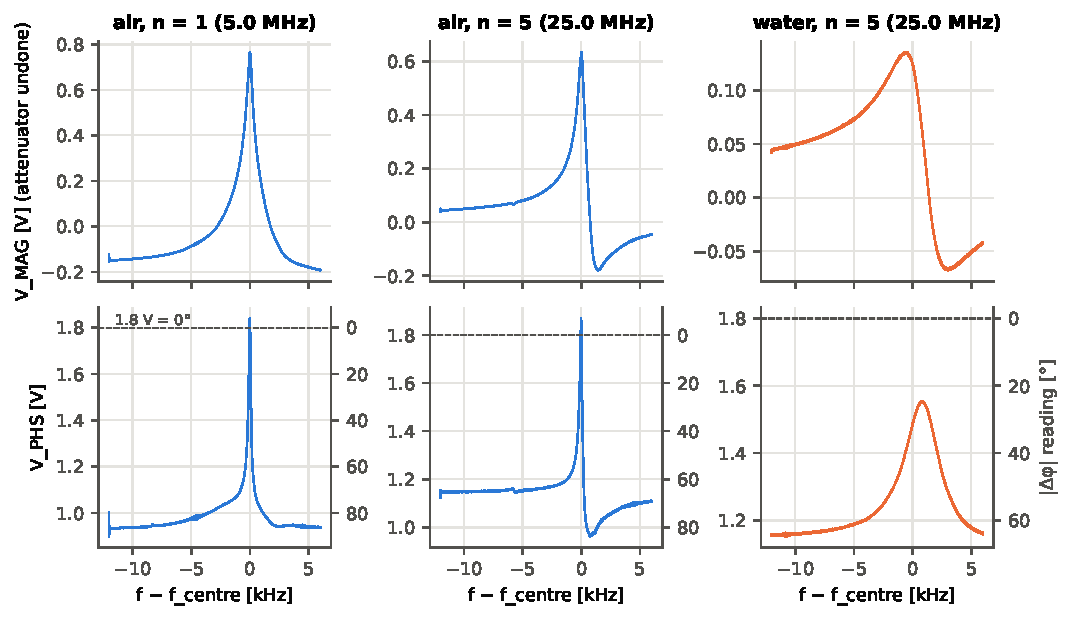
\includegraphics[width=\linewidth]{figures/si/fig02_raw_sweeps.pdf}
\caption{Raw detector voltages for the fundamental and the 5th overtone in air and for the 5th overtone in water (DS-2). Right axis: the unsigned phase reading. In air the reading folds at zero and overshoots it (the signature of $\delta$); in water it does not reach zero.}
\end{figure}

\begin{figure}[htbp]\centering
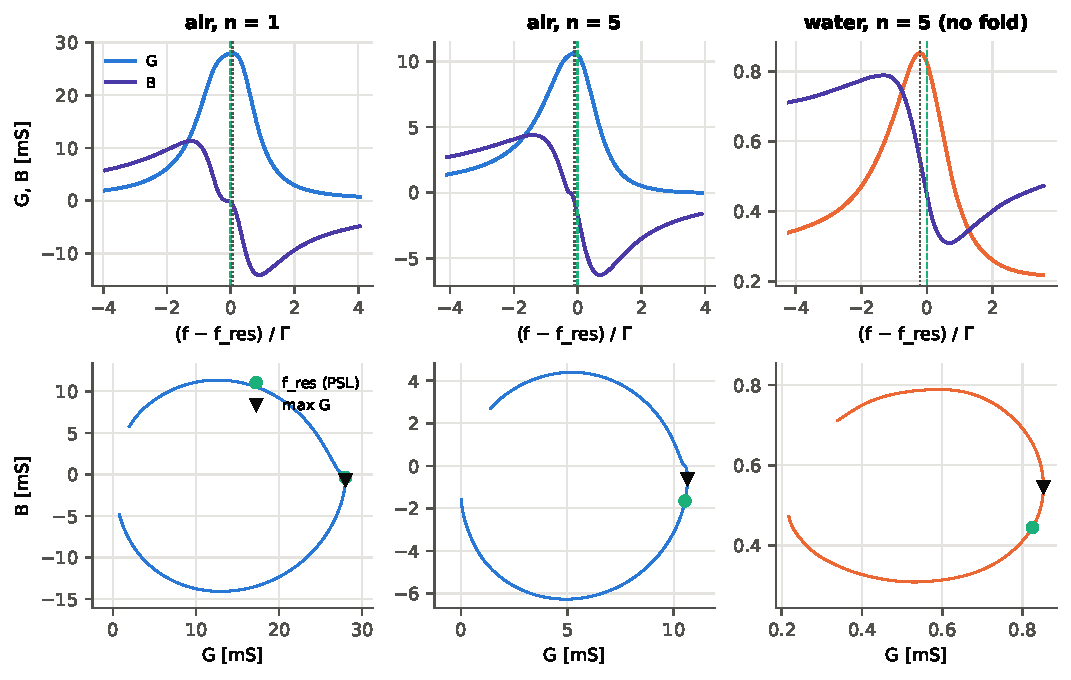
\includegraphics[width=\linewidth]{figures/si/fig03_G_B_locus.pdf}
\caption{Reconstructed conductance and susceptance (top) and admittance locus (bottom) on $\pm$4 $\Gamma$ for the sweeps of Fig. S1. Dotted: the maximum of $G$; marker: $f_\mathrm{res}$ of the phase-shifted fit.}
\end{figure}

\section{Closed-form biases of the simple estimators for a rotated Lorentzian}

With $\Delta = f_\mathrm{res} - f$ and $G - G_\mathrm{off} = A(\Gamma\cos\varphi - \Delta\sin\varphi)/(\Delta^2 + \Gamma^2)$, $dG/d\Delta = 0 \iff \sin\varphi\,\Delta^2 - 2\Gamma\cos\varphi\,\Delta - \Gamma^2\sin\varphi = 0$, whose maximum is $\Delta_\mathrm{max} = \Gamma(\cos\varphi - 1)/\sin\varphi = -\Gamma\tan(\varphi/2)$, hence $f_{G\max} = f_\mathrm{res} + \Gamma\tan(\varphi/2)$. The peak height above $G_\mathrm{off}$ is $(A/\Gamma)\cos^2(\varphi/2)$ and the curve has a negative lobe $-(A/\Gamma)\sin^2(\varphi/2)$ at $\Delta = \Gamma/\tan(\varphi/2)$. The half-height crossings (level $G_\mathrm{off}$ + half the peak height, $c = \cos^2(\varphi/2)$) solve $c\Delta^2 + 2\Gamma\sin\varphi\,\Delta + \Gamma^2(c - 2\cos\varphi) = 0$, $\Delta_\pm = \Gamma[-\sin\varphi \pm \sqrt{c(2-c)}]/c$, so $\Gamma_\mathrm{hh} = (\Delta_+ - \Delta_-)/2 = \Gamma\sqrt{(2-c)/c} = \Gamma\sqrt{1 + 2\tan^2(\varphi/2)}$ and $f_\mathrm{mid} = f_\mathrm{res} + 2\Gamma\tan(\varphi/2)$. Checked on noise-free model curves on the 1 Hz grid (\texttt{results/closed\_forms\_check.csv}): argmax bias numerical/theory $-$3.0/$-$2.8 Hz ($\varphi$ = $-$5\textdegree{}, $\Gamma$ = 65 Hz) \ldots{} $-$582/$-$582 Hz ($-$40\textdegree{}, 1600 Hz); $\Gamma$\_hh/$\Gamma$ 1.0014/1.0019 \ldots{} 1.1198/1.1247; midpoint $-$5.7/$-$5.7 \ldots{} $-$1048/$-$1165 Hz (the midpoint deviates from its closed form at large |$\varphi$| because the grid and the window truncate the far crossing). A symmetric Lorentzian with constant background fitted to a rotated one is biased by 1.9--2.1 $\Gamma$ tan($\varphi$/2) in frequency and over-estimates $\Gamma$ by 2--35 \% between $-$8\textdegree{} and $-$28\textdegree{}; with a linear background $\Gamma$ is right to 0.2 \% and the frequency bias is $\approx$1.25 $\Gamma$ tan($\varphi$/2).

\textbf{Sign convention.} Johannsmann et al. print Eq. 13 with $+\Delta\sin\varphi$ in $G$ and $+\Delta\cos\varphi$ in $B$; with one $\varphi$ in both lines that is not a single rotation (the lines correspond to $\varphi$ and $-\varphi$). Fitting $G$ alone, the two conventions are observationally identical and differ only in the sign quoted for $\varphi$; the main text uses the rotation form, in which the fitted angle is negative on both boards and the maximum of $G$ lies below $f_\mathrm{res}$. On the data the measured $f_{G\max} - f_\mathrm{res}$ is negative on every liquid sweep and on every air sweep with $n \ge 3$ (Table S8), as the convention requires.

\begin{figure}[htbp]\centering
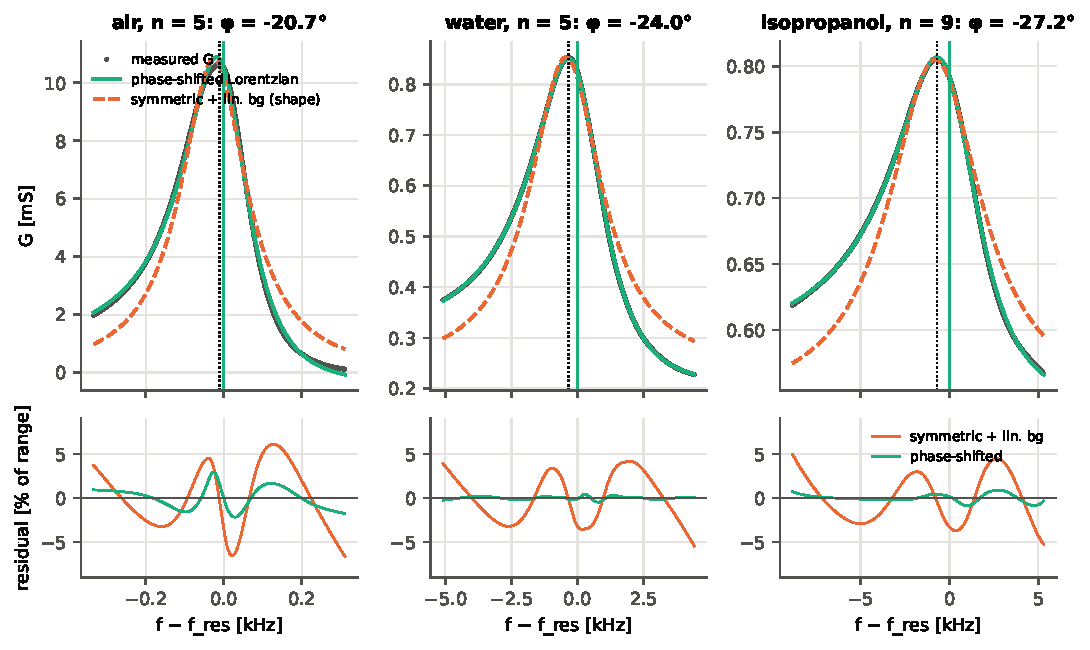
\includegraphics[width=\linewidth]{figures/si/fig04_fits_residuals.pdf}
\caption{Conductance (dots) with the phase-shifted Lorentzian (solid) and the symmetric Lorentzian with linear background (dashed) on $\pm$3 $\Gamma$\_hh for three sweeps of DS-2; below, the residuals in percent of the range of $G$.}
\end{figure}

\section{Fitting: window, initialisation, acceptance gate, fallback rate, residuals, repeatability}

Window $|f - f_{G\max}| \le 3\Gamma_\mathrm{hh}$ (clipped by the sweep edge on the right for $n \ge 5$ in isopropanol, 2.2--3.0 $\Gamma$ available, and at $n = 9$ in DS-3, 2.8--2.9 $\Gamma$ in water and 2.5--2.6 $\Gamma$ in the glucose solutions); seeds $f_{G\max}$, $\Gamma_\mathrm{hh}$, $\varphi = 0$, $G_\mathrm{off} = \min G$, $G_\mathrm{max}$ = range of $G$; frequencies scaled to kHz about the seed and conductances to mS; Levenberg--Marquardt with tolerances 10$^{-12}$. Gate (instrument constants): convergence, $f_\mathrm{res}$ inside the window, $0.3 \le \Gamma/\Gamma_\mathrm{hh} \le 3$, $|\varphi| \le 60^\circ$, rms residual $\le$ 5 \% of the range; the limits were set at about ten times the observed values on DS-2 and never fired: 45/45 fits of DS-2 and 75/75 of DS-3 converged and were accepted (fallback rate 0 \%). Residuals (rms, percent of the range of $G$): phase-shifted 1.0--2.7 \% in air and 0.15--0.65 \% in liquid on DS-2, 0.9--1.4 \% and 0.2--0.8 \% on DS-3; symmetric Lorentzian with linear background 3.0--4.2 \% and 0.8--3.5 \% (DS-2), 1.8--4.2 \% and 0.7--3.8 \% (DS-3), always S-shaped (Fig. S3). The fit's covariance gives 0.1--0.8 Hz on $f_\mathrm{res}$, an order of magnitude below the replica scatter, because the residual is structured; the replica scatter is the number quoted. Repeatability over the three sweeps of a plateau (Fig. S4): DS-2, $f_\mathrm{res}$ 1.5--23 Hz in air (the air baseline was still drifting at $-$0.3 to $-$2 Hz/min) and 0.3--29 Hz in liquid, $\Gamma$ $\le$ 2.3 Hz in air and $\le$ 38 Hz in liquid (the two-state sweep; $\le$ 13 Hz otherwise); DS-3, $f_\mathrm{res}$ $\le$ 2.4 Hz in air and $\le$ 7.6 Hz in liquid, $\Gamma$ $\le$ 0.7 and $\le$ 4.5 Hz. The magnitude estimator's $-$3 dB width is undefined inside the window on 15 of 45 (DS-2) and 33 of 75 (DS-3) sweeps; the half-height width of $G$ is two-sided on all 120.

\begin{figure}[htbp]\centering
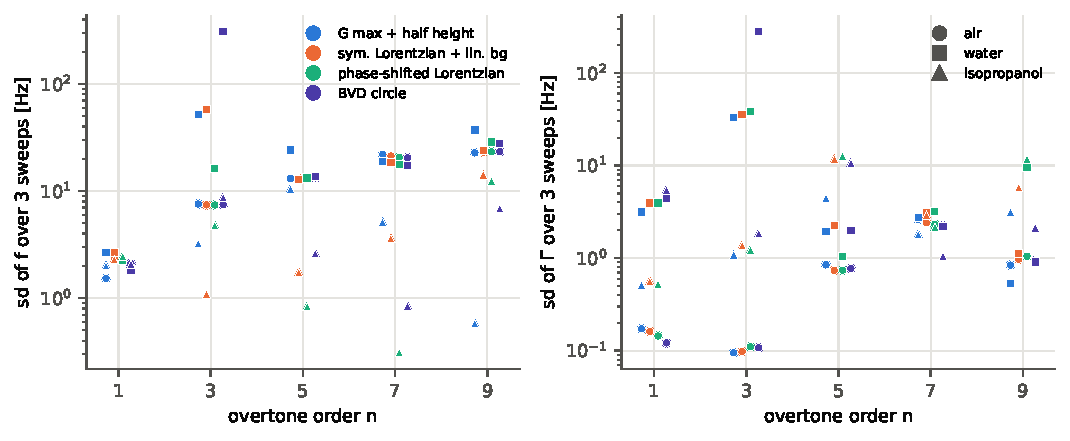
\includegraphics[width=\linewidth]{figures/si/fig09_repeatability.pdf}
\caption{Standard deviation over the three plateau sweeps of $f_\mathrm{res}$ (left) and $\Gamma$ (right) per estimator, overtone and load, DS-2.}
\end{figure}

\section{Forward model, board phase, resistive standards}

A board phase does not multiply the admittance; it multiplies the measured transfer function, $H_\mathrm{meas} = He^{j\phi_b}$. Inverting exactly with that phase gives $Y' = 1/[(Z_\mathrm{el} + R_{17})e^{-j\phi_b} - R_{17}]$, a Möbius transformation of $Y_\mathrm{el} = 1/Z_\mathrm{el}$ that reduces to the rotation $Y_\mathrm{el}e^{j\phi_b}$ only when $|Z_\mathrm{el}| \gg R_{17}$. A Butterworth--Van Dyke crystal of known $f_s$, $\Gamma$, $R_1$, $C_0$ was sent through the divider and the detector laws with a board phase on $\angle H$, an offset $\delta$, the fold, the ADC quantisation and the firmware carry-over, and through the same chain and estimators (\texttt{run\_forward\_model.py}, \texttt{results/forward\_model.md}). Findings: (i) the fitted angle equals the imposed board phase to 0.7\textdegree{} on the liquid-like cases and to 1\textdegree{} on the air-like ones, except the one case where the offset triggers a spurious fold; (ii) with $\phi_b = 0$ both estimators recover $f_s$ to the grid; (iii) with $\phi_b = -8$ to $-25^\circ$ the maximum of $G$ is off by $-$91 to $-$743 Hz on liquid-like cases, the phase-shifted fit by $-$9 to $-$59 Hz ($\le$2 \% of $\Gamma$), the symmetric fit by $-$96 to $-$833 Hz; (iv) the residual of the phase-shifted fit scales as $\approx -0.34\,\Gamma\,(R_{17}/R_1)$ at $\phi_b = -20^\circ$: $-$344 Hz at $R_1 = R_{17}$ and $-$12 Hz at 1.6 k$\Omega$ for $\Gamma$ = 1 kHz, so for air-like cases ($\Gamma$ = 65--190 Hz, $R_1$ = 36--204 $\Omega$) $-$12 to $-$39 Hz, a third to a half of the argmax bias for $R_1/R_{17} \ge 1.8$ and three quarters or more at $R_1/R_{17}$ = 0.7; (v) with a fold, $\delta$ is removed and does not move $f_\mathrm{res}$ or $\Gamma$ ($\le$0.5 Hz for $\delta$ = $-$3\ldots{}+7\textdegree{}); (vi) without a fold, $\pm$5\textdegree{} of $\delta$ enters the fitted angle almost one to one and moves $f_\mathrm{res}$ by $\le$11 Hz (15 Hz where a spurious fold is declared) and $\Gamma$ by $\le$7 Hz; (vii) $\pm$5 \% on the magnitude slope moves $f_\mathrm{res}$ by $\le$17 Hz and $\Gamma$ by $\le$1 \%, but $R_m = 1/G_\mathrm{max}$ by 6--16 \%, and even with an ideal magnitude channel $R_m$ is 24--39 \% low in liquid; (viii) the firmware carry-over moves $f_\mathrm{res}$ by $\approx$2 Hz; (ix) the smoothing widens a 65 Hz half-bandwidth by 6.5 Hz (+10 \%) and a 190 Hz one by 3.5 Hz, negligible in liquid.

The repository's two-channel forward model, which fits a BVD crystal through the divider and the detector laws to $V_\mathrm{MAG}$ and $V_\mathrm{PHS}$ jointly with a board phase inside the modulus, gives $\phi_b = -7.6, -13.8, -19.9, -22.1, -20.4^\circ$ in air on board 1920, equal to the P angle within 0.4--0.8\textdegree{} on $n = 1$--7. The short and 50 $\Omega$ standards measured on the same front end (1--51 MHz) give phase slopes of 0.27--0.40\textdegree{} MHz$^{-1}$ (0.74--1.10 ns), i.e. 1.4--2.0\textdegree{} at 5 MHz and 12--18\textdegree{} at 45 MHz, and read $M$ 4--16 \% low (8--14 \% at 5 MHz); the fitted angle grows roughly as $f^{0.55}$ (Fig. S11). A least-squares decomposition $\varphi = \varphi_0 - 360^\circ f\tau$ gives $\varphi_0 = -7.0^\circ$, $\tau$ = 1.28 ns (rms 1.2\textdegree{}) for board 1920 in air and $\varphi_0 = -8.2^\circ$, $\tau$ = 1.31 ns (rms 2.6\textdegree{}) for the second instrument, an approximation whose parameters move when $n = 1$ is excluded.

\begin{figure}[htbp]\centering
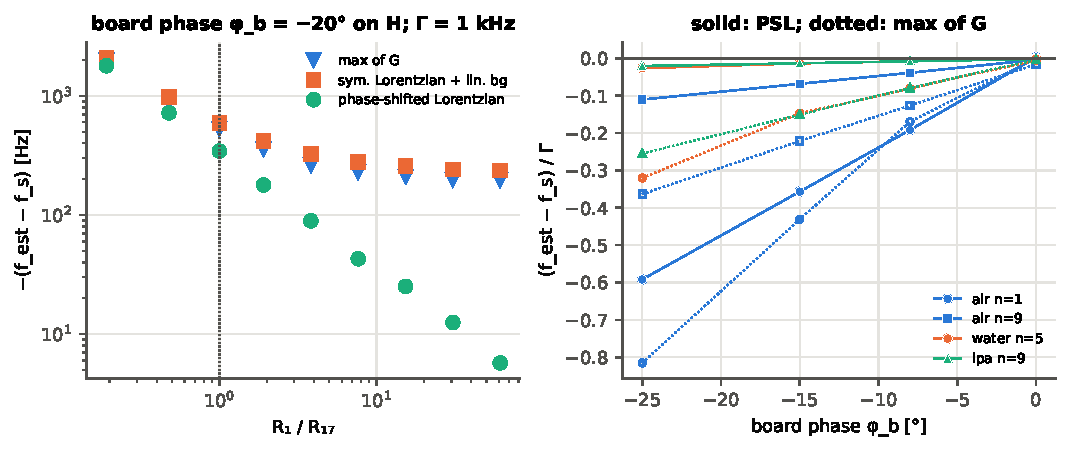
\includegraphics[width=\linewidth]{figures/si/fig10_forward_model.pdf}
\caption{Forward model. Left: error of three estimators against $R_1/R_{17}$ for a board phase of $-$20\textdegree{} on the transfer function ($\Gamma$ = 1 kHz). Right: error in units of $\Gamma$ against the board phase for four measured-like cases; solid: phase-shifted fit; dotted: maximum of $G$.}
\end{figure}

\section{Firmware carry-over}

Firmware versions up to 0.1.5c did not reset the per-point sums, so each printed point carried 1/500 of the previous one (+0.2 \% on the counts). The recursion is exact and was undone offline on the counts ($m_i = v_i - v_{i-1}/500$). On DS-2 it changes $f_\mathrm{res}$ by $\le$2.2 Hz and $\Gamma$ by $\le$1.7 Hz on 43 of 45 sweeps with P and $\varphi$ by $\le$0.2\textdegree{}; the exceptions are the threshold sweep of S3, whose fold decision flips ($f_\mathrm{res}$ +37 Hz with P, +111 Hz with A; $\varphi$ +4.3\textdegree{}), and one water sweep at $n$ = 9 (+10 Hz on $f_\mathrm{res}$, $-$18 Hz on $\Gamma$). With A the changes are larger ($\le$2 Hz on 21 of 45 sweeps, up to 111 Hz). On DS-3 it changes $f_\mathrm{res}$ by $\le$2 Hz (P; $\le$6 Hz with A), $\Gamma$ by $\le$2 Hz and $\varphi$ by $\le$0.2\textdegree{}. Over the 120 sweeps the fit moves by $\le$2 Hz on 115 and by $\le$4 Hz on 118. The A and P ranges of Table 2 move by $\le$2 percentage points (the M rows by up to 3.4) (corrected variant: DS-2 P $\epsilon_f$ = $-$1.6\ldots{}+7.8 \%, $\epsilon_\Gamma$ = $-$4.3\ldots{}+7.3 \%; DS-3 P +6.0\ldots{}+13.0 \%, $-$4.4\ldots{}+4.6 \%); the bias law gives +14 $\pm$ 30 Hz on 120 sweeps. Fig. S6 shows the differences on the shifts.

\begin{figure}[htbp]\centering
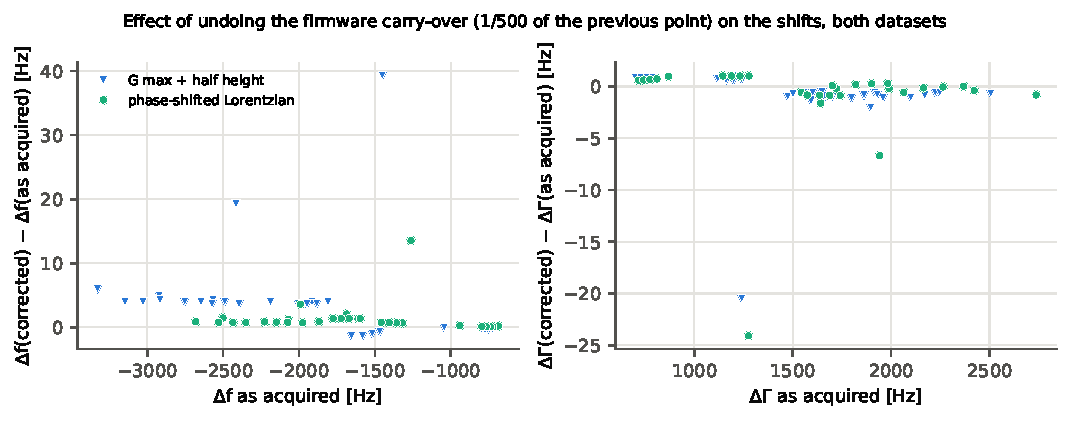
\includegraphics[width=\linewidth]{figures/si/figS_firmware_correction.pdf}
\caption{Difference of the air-to-liquid shifts between the firmware-corrected and the as-acquired variants, both datasets, estimators A and P.}
\end{figure}

\section{The raw-magnitude baseline and the production datalogs}

\textbf{Magnitude-only estimator from the sweeps (M).} Maximum of the divider ratio in dB on the same grid and its $-$3 dB full width where it exists (Table S3 and Fig. S7): $\epsilon_f$ = +52\ldots{}+92 \% (DS-2) and +50\ldots{}+116 \% (DS-3) on $n$ = 3--9, growing with the overtone; the width is undefined inside the window for $n \ge 7$ in liquid and reaches 6 kHz at $n$ = 5. \textbf{Production datalog of board 1920} (same instants as the impedance datalog, Fig. S8): maximum of the baseline-corrected magnitude and its $-$0.3 dB width; on the last 10 min of each plateau of 2026-09-11 (95 of 486 rows were exact duplicates written in bursts and were dropped) $\epsilon_f$ = +51, +69, +76, +89 \% (water, $n$ = 3--9) and +57, +74, +85, +90 \% (isopropanol), against +23, +29, +22, +18 \% and +22, +27, +22, +22 \% for the live A estimator; the $-$0.3 dB width changes by 0.8--3.7 kHz (water) and 1.1--6.4 kHz (isopropanol) where the theory's $\Delta$$\Gamma$ is 1.2--2.7 kHz. The 2026-09-10 run (2.5 min plateaus, 36 of 175 rows duplicated) gives +51\ldots{}+98 \% and +22\ldots{}+30 \%. The live A estimator reproduces the offline analysis of the dumped sweeps within the plateau drift (Table S11).

\begin{figure}[htbp]\centering
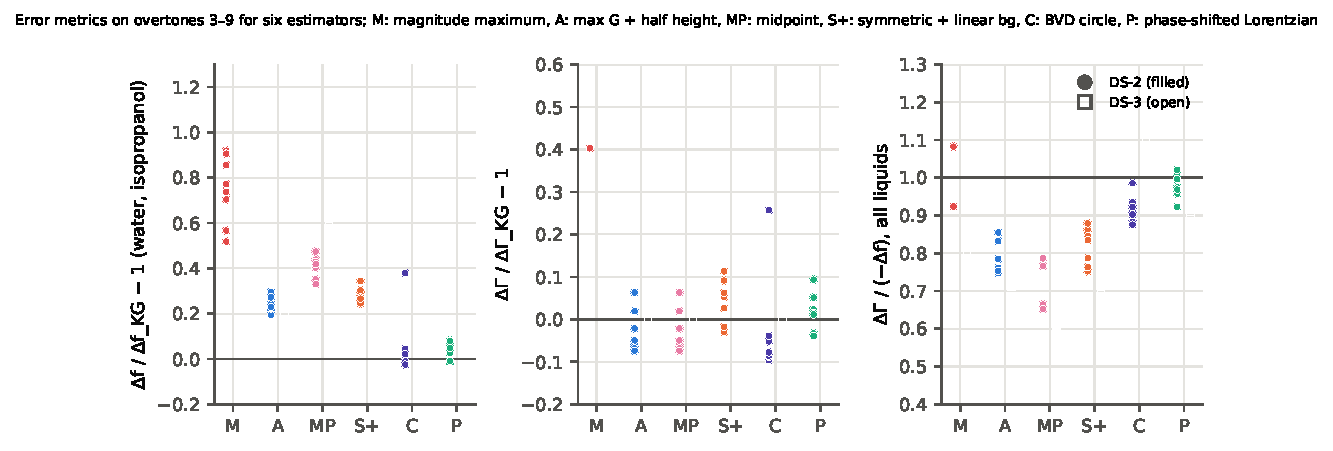
\includegraphics[width=\linewidth]{figures/si/figS_estimator_errors.pdf}
\caption{Error metrics on overtones 3--9 for six estimators on both datasets: $\epsilon_f$, $\epsilon_\Gamma$ (water and isopropanol) and $r_n$ (all liquids).}
\end{figure}

\begin{figure}[htbp]\centering
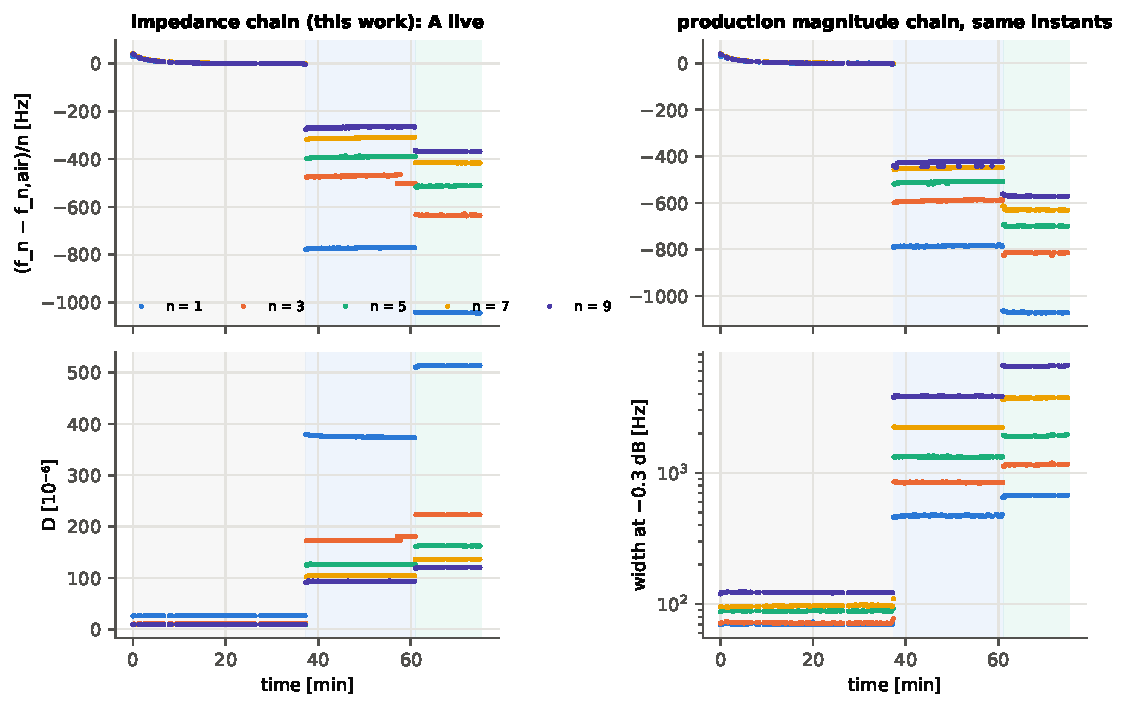
\includegraphics[width=\linewidth]{figures/si/figS_datalogs_0911.pdf}
\caption{The run of 2026-09-11 as logged by the instrument: the impedance chain (left; A live) and the production magnitude chain at the same instants (right); overtone-normalised frequency relative to the air plateau, dissipation factor, and the production $-$0.3 dB width.}
\end{figure}

\section{Glucose series: concentration lines, the 5 \% offset, the fit window}

Relative to water, the fitted resonance moves by $-$72 Hz (fundamental) to $-$307 Hz (9th) at 10 \% w/v ($-$17 to $-$128 Hz at 5 \%) and broadens by +94 to +379 Hz at 10 \%; lines through the four concentrations have slopes $-$7.1, $-$13.8, $-$17.8, $-$24.7, $-$30.4 Hz per \% w/v in $\Delta f_n$ and +9.2, +13.1, +16.6, +28.0, +37.8 Hz per \% in $\Delta\Gamma_n$ (Fig. S9). The 5 \% plateau is less loaded than the line on every overtone: +10 to +18 Hz in $\Delta$f and $-$9 to $-$14 Hz in $\Delta$$\Gamma$, constant in hertz over $n$ rather than $\propto$ $\surd$n, so not an error of $\rho$$\eta$. Drift cannot explain it: the slope of $f_\mathrm{res}$ over the three replicas is $\le$0.4 Hz/min inside the glucose plateaus and $-$0.2 to $-$1.0 Hz/min in water, the 5 \% plateau is 4.3 min off the line of plateau times against concentration, so a time-linear drift maps into at most $\approx$4 Hz, and explaining the residual by drift alone would need $-$2 to $-$4 Hz/min, three to sixteen times what is measured (\texttt{results/glucose\_tables\_asis.md}). Without a return to water between concentrations the experiment cannot tell a property of the first solution from a step of the instrument. The ratio $\rho\eta/(\rho\eta)_w$ from the bandwidth exceeds that from the frequency on $n$ = 7 and 9 (1.36 and 1.42 against 1.27 and 1.30 at 10 \%); the $\pm$3$\Gamma$ fit window is clipped by the sweep edge there (2.5--2.6 $\Gamma$ on the right at $n$ = 9), and refitting with a symmetric window limited by the edge moves the $n$ = 9 ratio from 1.418 to 1.395, a fifth of the gap, and nothing at $n$ = 7; the rest is unexplained. A roughness term, which in the Daikhin--Urbakh description adds to $\Delta$f without a counterpart in $\Delta$$\Gamma$ \citep{DaikhinUrbakh1996, DaikhinUrbakh1997}, would act in the opposite direction and is not supported.

\begin{figure}[htbp]\centering
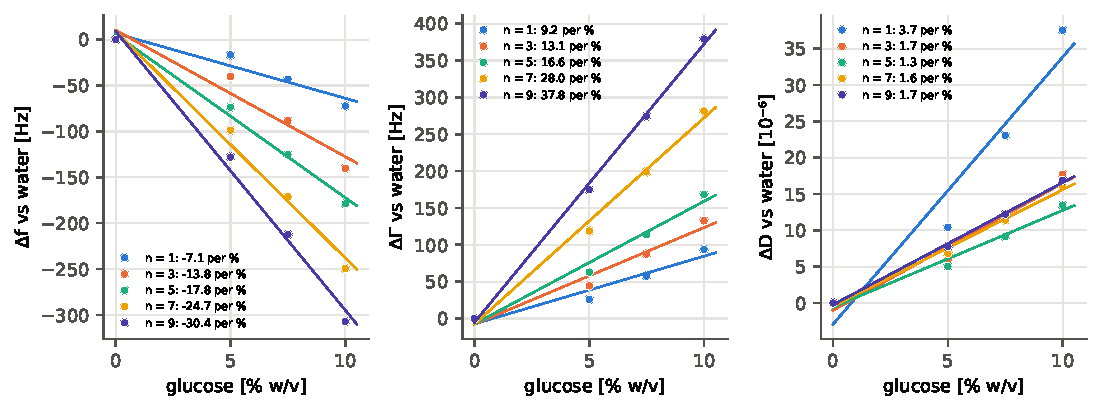
\includegraphics[width=\linewidth]{figures/si/figS_glucose_lines.pdf}
\caption{Shifts relative to water of the fitted resonance frequency, half-bandwidth and dissipation against glucose concentration, one line per overtone (least squares with intercept).}
\end{figure}

\begin{figure}[htbp]\centering
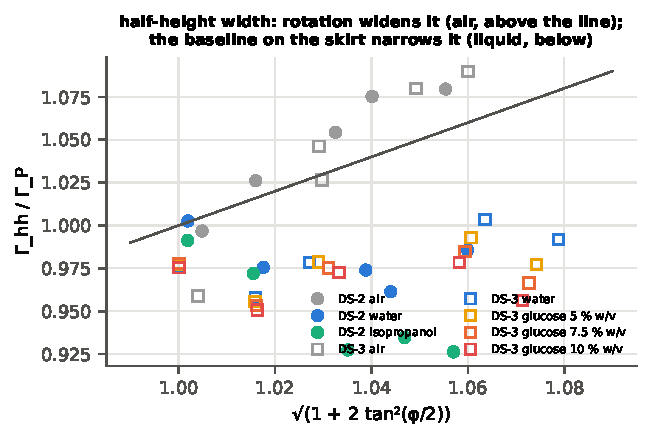
\includegraphics[width=\linewidth]{figures/si/figS_halfheight_width.pdf}
\caption{The half-height width against the fitted $\Gamma$: rotation widens it (air, above the identity), the baseline on the skirt narrows it (liquid, below).}
\end{figure}

\begin{figure}[htbp]\centering
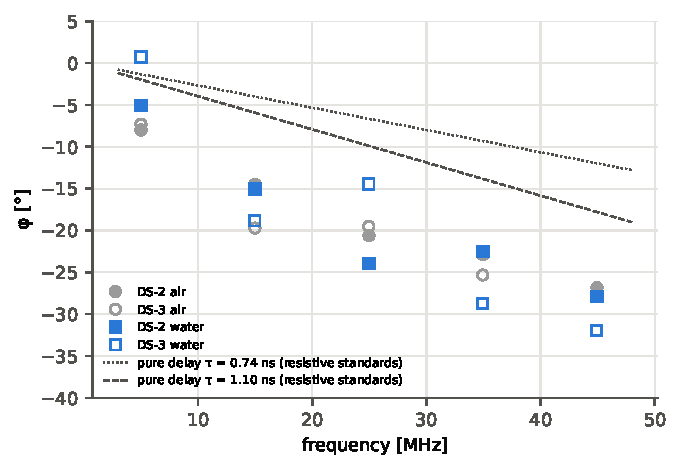
\includegraphics[width=\linewidth]{figures/si/figS_phi_vs_frequency.pdf}
\caption{The rotation angle against frequency for air and water on both instruments, with the phase of a pure delay for the two delays measured on the resistive standards of board 1920.}
\end{figure}

\begin{figure}[htbp]\centering
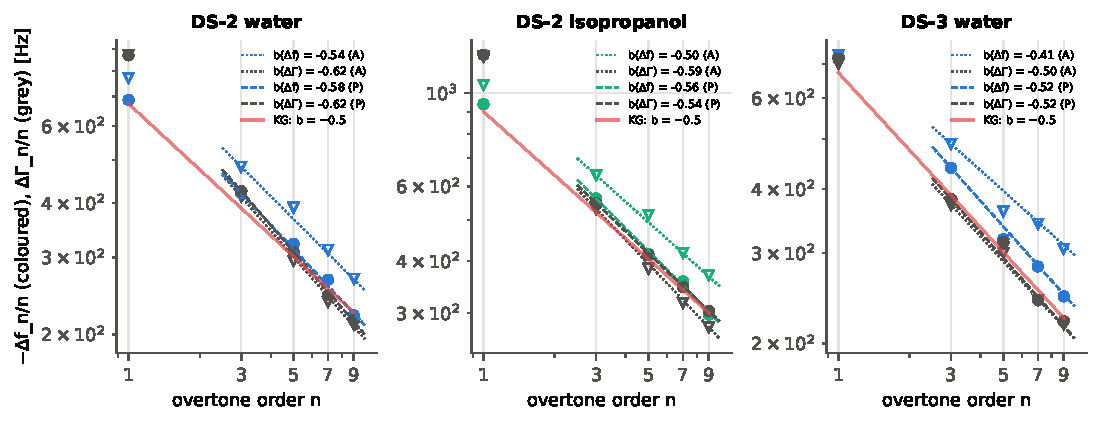
\includegraphics[width=\linewidth]{figures/si/figS_kg2_loglog.pdf}
\caption{KG-2 on log--log axes: $-\Delta f_n/n$ and $\Delta\Gamma_n/n$ against $n$ for A and P with the fitted slopes on $n$ = 3--9 and the KG line of slope $-$1/2.}
\end{figure}

\section{Tables}

\begin{landscape}{\scriptsize\setlength{\tabcolsep}{2pt}
\begin{longtable}{@{}lllllllllll@{}}
\caption{Resonance frequency, half-bandwidth, dissipation and rotation angle per dataset, medium and overtone (mean $\pm$ sd of three sweeps). A = maximum of $G$ + half height; P = phase-shifted Lorentzian; fold = number of sweeps on which the phase reading folds.}\\
\toprule
dataset & medium & n & f (A) [Hz] & f (P) [Hz] & $\Gamma$ (A) [Hz] & $\Gamma$ (P) [Hz] & D (A) [10$^{-6}$] & D (P) [10$^{-6}$] & $\varphi$ (P) [\textdegree{}] & fold \\\midrule\endhead
DS-2 & air & 1 & 5004598 $\pm$ 2 & 5004596 $\pm$ 2 & 65.4 $\pm$ 0.2 & 65.6 $\pm$ 0.1 & 26.1 & 26.2 & -8.0 $\pm$ 0.05 & 3/3 \\
DS-2 & air & 3 & 14988738 $\pm$ 8 & 14988740 $\pm$ 7 & 78.0 $\pm$ 0.1 & 76.0 $\pm$ 0.1 & 10.4 & 10.1 & -14.5 $\pm$ 0.03 & 3/3 \\
DS-2 & air & 5 & 24973688 $\pm$ 13 & 24973699 $\pm$ 13 & 108.0 $\pm$ 0.8 & 102.4 $\pm$ 0.7 & 8.6 & 8.2 & -20.6 $\pm$ 0.06 & 3/3 \\
DS-2 & air & 7 & 34957566 $\pm$ 22 & 34957593 $\pm$ 21 & 158.7 $\pm$ 2.6 & 147.6 $\pm$ 2.3 & 9.1 & 8.4 & -22.9 $\pm$ 0.04 & 3/3 \\
DS-2 & air & 9 & 44943110 $\pm$ 23 & 44943157 $\pm$ 23 & 203.7 $\pm$ 0.8 & 188.7 $\pm$ 1.0 & 9.1 & 8.4 & -26.8 $\pm$ 0.00 & 3/3 \\
DS-2 & water & 1 & 5003826 $\pm$ 3 & 5003909 $\pm$ 2 & 937.0 $\pm$ 3.2 & 934.5 $\pm$ 3.9 & 374.5 & 373.5 & -5.0 $\pm$ 0.02 & 3/3 \\
DS-2 & water & 3 & 14987288 $\pm$ 52 & 14987478 $\pm$ 16 & 1318.2 $\pm$ 33.1 & 1351.4 $\pm$ 38.2 & 175.9 & 180.3 & -15.0 $\pm$ 2.45 & 1/3 \\
DS-2 & water & 5 & 24971737 $\pm$ 24 & 24972088 $\pm$ 13 & 1582.0 $\pm$ 2.0 & 1645.6 $\pm$ 1.0 & 126.7 & 131.8 & -24.0 $\pm$ 0.04 & 0/3 \\
DS-2 & water & 7 & 34955379 $\pm$ 19 & 34955726 $\pm$ 18 & 1822.9 $\pm$ 2.8 & 1871.6 $\pm$ 3.2 & 104.3 & 107.1 & -22.5 $\pm$ 0.05 & 0/3 \\
DS-2 & water & 9 & 44940695 $\pm$ 37 & 44941165 $\pm$ 29 & 2099.7 $\pm$ 0.5 & 2130.1 $\pm$ 9.6 & 93.4 & 94.8 & -27.9 $\pm$ 0.23 & 0/3 \\
DS-2 & isopropanol & 1 & 5003555 $\pm$ 2 & 5003656 $\pm$ 2 & 1285.6 $\pm$ 0.5 & 1296.9 $\pm$ 0.5 & 513.9 & 518.4 & -5.0 $\pm$ 0.02 & 3/3 \\
DS-2 & isopropanol & 3 & 14986825 $\pm$ 3 & 14987054 $\pm$ 5 & 1670.5 $\pm$ 1.1 & 1718.6 $\pm$ 1.2 & 222.9 & 229.3 & -14.2 $\pm$ 0.18 & 0/3 \\
DS-2 & isopropanol & 5 & 24971122 $\pm$ 10 & 24971627 $\pm$ 1 & 2025.1 $\pm$ 4.4 & 2166.8 $\pm$ 12.6 & 162.2 & 173.5 & -24.7 $\pm$ 0.17 & 0/3 \\
DS-2 & isopropanol & 7 & 34954645 $\pm$ 5 & 34955093 $\pm$ 0 & 2383.2 $\pm$ 1.8 & 2569.8 $\pm$ 2.2 & 136.4 & 147.0 & -21.4 $\pm$ 0.11 & 0/3 \\
DS-2 & isopropanol & 9 & 44939783 $\pm$ 1 & 44940476 $\pm$ 12 & 2709.8 $\pm$ 3.1 & 2925.5 $\pm$ 11.6 & 120.6 & 130.2 & -27.2 $\pm$ 0.04 & 0/3 \\
DS-3 & air & 1 & 5000106 $\pm$ 1 & 5000107 $\pm$ 1 & 110.0 $\pm$ 0.7 & 114.7 $\pm$ 0.7 & 44.0 & 45.9 & -7.3 $\pm$ 0.13 & 3/3 \\
DS-3 & air & 3 & 14977476 $\pm$ 0 & 14977481 $\pm$ 0 & 52.6 $\pm$ 0.1 & 51.3 $\pm$ 0.1 & 7.0 & 6.8 & -19.7 $\pm$ 0.02 & 3/3 \\
DS-3 & air & 5 & 24955252 $\pm$ 1 & 24955258 $\pm$ 1 & 70.0 $\pm$ 0.1 & 66.9 $\pm$ 0.1 & 5.6 & 5.4 & -19.5 $\pm$ 0.02 & 3/3 \\
DS-3 & air & 7 & 34931726 $\pm$ 2 & 34931742 $\pm$ 2 & 106.2 $\pm$ 0.3 & 98.3 $\pm$ 0.2 & 6.1 & 5.6 & -25.3 $\pm$ 0.05 & 3/3 \\
DS-3 & air & 9 & 44909699 $\pm$ 3 & 44909726 $\pm$ 2 & 152.3 $\pm$ 0.1 & 139.8 $\pm$ 0.1 & 6.8 & 6.2 & -27.9 $\pm$ 0.05 & 3/3 \\
DS-3 & water & 1 & 4999377 $\pm$ 3 & 4999384 $\pm$ 1 & 811.1 $\pm$ 1.4 & 831.0 $\pm$ 1.5 & 324.5 & 332.5 & 0.7 $\pm$ 0.03 & 3/3 \\
DS-3 & water & 3 & 14976009 $\pm$ 3 & 14976163 $\pm$ 3 & 1170.8 $\pm$ 1.3 & 1196.4 $\pm$ 1.9 & 156.4 & 159.8 & -18.8 $\pm$ 0.03 & 3/3 \\
DS-3 & water & 5 & 24953443 $\pm$ 5 & 24953662 $\pm$ 4 & 1571.3 $\pm$ 1.1 & 1640.4 $\pm$ 0.6 & 125.9 & 131.5 & -14.4 $\pm$ 0.02 & 0/3 \\
DS-3 & water & 7 & 34929332 $\pm$ 3 & 34929765 $\pm$ 5 & 1806.6 $\pm$ 2.3 & 1800.1 $\pm$ 0.1 & 103.4 & 103.1 & -28.7 $\pm$ 0.01 & 0/3 \\
DS-3 & water & 9 & 44906947 $\pm$ 36 & 44907503 $\pm$ 8 & 2111.9 $\pm$ 2.4 & 2129.1 $\pm$ 4.5 & 94.1 & 94.8 & -31.9 $\pm$ 0.03 & 0/3 \\
DS-3 & glucose 5 \% & 1 & 4999359 $\pm$ 2 & 4999367 $\pm$ 0 & 837.5 $\pm$ 0.4 & 857.1 $\pm$ 0.8 & 335.0 & 342.9 & 0.9 $\pm$ 0.01 & 3/3 \\
DS-3 & glucose 5 \% & 3 & 14975959 $\pm$ 2 & 14976123 $\pm$ 0 & 1214.3 $\pm$ 0.2 & 1240.7 $\pm$ 0.2 & 162.2 & 165.7 & -19.5 $\pm$ 0.01 & 3/3 \\
DS-3 & glucose 5 \% & 5 & 24953369 $\pm$ 3 & 24953588 $\pm$ 1 & 1627.6 $\pm$ 2.4 & 1703.3 $\pm$ 0.5 & 130.5 & 136.5 & -14.4 $\pm$ 0.00 & 0/3 \\
DS-3 & glucose 5 \% & 7 & 34929237 $\pm$ 4 & 34929667 $\pm$ 1 & 1905.2 $\pm$ 0.8 & 1918.9 $\pm$ 0.3 & 109.1 & 109.9 & -28.1 $\pm$ 0.01 & 0/3 \\
DS-3 & glucose 5 \% & 9 & 44906784 $\pm$ 7 & 44907375 $\pm$ 1 & 2251.6 $\pm$ 4.0 & 2303.8 $\pm$ 0.8 & 100.3 & 102.6 & -31.0 $\pm$ 0.04 & 0/3 \\
DS-3 & glucose 7.5 \% & 1 & 4999332 $\pm$ 3 & 4999341 $\pm$ 0 & 869.0 $\pm$ 0.2 & 888.7 $\pm$ 0.9 & 347.6 & 355.5 & 1.1 $\pm$ 0.01 & 3/3 \\
DS-3 & glucose 7.5 \% & 3 & 14975895 $\pm$ 4 & 14976075 $\pm$ 1 & 1252.1 $\pm$ 0.3 & 1284.0 $\pm$ 0.5 & 167.2 & 171.5 & -20.2 $\pm$ 0.01 & 3/3 \\
DS-3 & glucose 7.5 \% & 5 & 24953306 $\pm$ 5 & 24953536 $\pm$ 1 & 1672.6 $\pm$ 1.8 & 1754.4 $\pm$ 0.8 & 134.1 & 140.6 & -14.5 $\pm$ 0.01 & 0/3 \\
DS-3 & glucose 7.5 \% & 7 & 34929154 $\pm$ 14 & 34929594 $\pm$ 1 & 1968.6 $\pm$ 1.1 & 1999.1 $\pm$ 0.2 & 112.7 & 114.5 & -27.8 $\pm$ 0.00 & 0/3 \\
DS-3 & glucose 7.5 \% & 9 & 44906672 $\pm$ 3 & 44907291 $\pm$ 0 & 2323.1 $\pm$ 5.7 & 2403.7 $\pm$ 1.4 & 103.5 & 107.1 & -30.7 $\pm$ 0.02 & 0/3 \\
DS-3 & glucose 10 \% & 1 & 4999304 $\pm$ 3 & 4999311 $\pm$ 0 & 902.1 $\pm$ 0.7 & 924.9 $\pm$ 0.9 & 360.9 & 370.0 & 1.2 $\pm$ 0.01 & 3/3 \\
DS-3 & glucose 10 \% & 3 & 14975822 $\pm$ 2 & 14976023 $\pm$ 0 & 1292.4 $\pm$ 0.9 & 1329.0 $\pm$ 0.8 & 172.6 & 177.5 & -20.8 $\pm$ 0.03 & 3/3 \\
DS-3 & glucose 10 \% & 5 & 24953248 $\pm$ 3 & 24953483 $\pm$ 1 & 1719.4 $\pm$ 1.6 & 1808.4 $\pm$ 0.8 & 137.8 & 144.9 & -14.6 $\pm$ 0.02 & 0/3 \\
DS-3 & glucose 10 \% & 7 & 34929080 $\pm$ 7 & 34929516 $\pm$ 1 & 2036.5 $\pm$ 0.9 & 2081.6 $\pm$ 2.2 & 116.6 & 119.2 & -27.5 $\pm$ 0.02 & 0/3 \\
DS-3 & glucose 10 \% & 9 & 44906553 $\pm$ 2 & 44907196 $\pm$ 3 & 2398.9 $\pm$ 2.4 & 2508.4 $\pm$ 1.2 & 106.8 & 111.7 & -30.4 $\pm$ 0.07 & 0/3 \\
\bottomrule
\end{longtable}}\end{landscape}

\begin{landscape}{\scriptsize\setlength{\tabcolsep}{2pt}
\begin{longtable}{@{}lllllllllllll@{}}
\caption{Air-to-liquid shifts for A and P, all datasets and liquids, with the three tests. $\epsilon$ only where $\rho$$\eta$ is tabulated (water, isopropanol).}\\
\toprule
dataset & liquid & n & est. & $\Delta$f [Hz] & $\Delta$f/n & $\Delta$$\Gamma$ [Hz] & $\Delta$$\Gamma$/n & $\Delta$f\_KG & $\epsilon$\_f [\%] & $\epsilon$\_$\Gamma$ [\%] & r = $\Delta$$\Gamma$/($-$$\Delta$f) & $\Delta$D [10$^{-6}$] \\\midrule\endhead
DS-2 & water & 1 & A & -772 $\pm$ 3 & -772 & 872 $\pm$ 3 & 872 & -674 & +14.7 & +29.4 & 1.129 & 348.4 \\
DS-2 & water & 3 & A & -1451 $\pm$ 52 & -484 & 1240 $\pm$ 33 & 413 & -1167 & +24.3 & +6.3 & 0.855 & 165.5 \\
DS-2 & water & 5 & A & -1951 $\pm$ 28 & -390 & 1474 $\pm$ 2 & 295 & -1506 & +29.5 & -2.1 & 0.756 & 118.1 \\
DS-2 & water & 7 & A & -2187 $\pm$ 29 & -312 & 1664 $\pm$ 4 & 238 & -1782 & +22.7 & -6.6 & 0.761 & 95.2 \\
DS-2 & water & 9 & A & -2415 $\pm$ 44 & -268 & 1896 $\pm$ 1 & 211 & -2021 & +19.5 & -6.2 & 0.785 & 84.4 \\
DS-2 & water & 1 & P & -687 $\pm$ 3 & -687 & 869 $\pm$ 4 & 869 & -674 & +2.0 & +29.0 & 1.265 & 347.3 \\
DS-2 & water & 3 & P & -1262 $\pm$ 18 & -421 & 1275 $\pm$ 38 & 425 & -1167 & +8.2 & +9.3 & 1.011 & 170.2 \\
DS-2 & water & 5 & P & -1611 $\pm$ 19 & -322 & 1543 $\pm$ 1 & 309 & -1506 & +7.0 & +2.5 & 0.958 & 123.6 \\
DS-2 & water & 7 & P & -1868 $\pm$ 27 & -267 & 1724 $\pm$ 4 & 246 & -1782 & +4.8 & -3.3 & 0.923 & 98.6 \\
DS-2 & water & 9 & P & -1991 $\pm$ 37 & -221 & 1941 $\pm$ 10 & 216 & -2021 & -1.4 & -3.9 & 0.975 & 86.4 \\
DS-2 & isopropanol & 1 & A & -1043 $\pm$ 3 & -1043 & 1220 $\pm$ 1 & 1220 & -902 & +15.7 & +35.3 & 1.169 & 487.7 \\
DS-2 & isopropanol & 3 & A & -1914 $\pm$ 8 & -638 & 1593 $\pm$ 1 & 531 & -1562 & +22.5 & +1.9 & 0.832 & 212.5 \\
DS-2 & isopropanol & 5 & A & -2566 $\pm$ 17 & -513 & 1917 $\pm$ 4 & 383 & -2017 & +27.2 & -5.0 & 0.747 & 153.5 \\
DS-2 & isopropanol & 7 & A & -2921 $\pm$ 23 & -417 & 2224 $\pm$ 3 & 318 & -2387 & +22.4 & -6.8 & 0.762 & 127.3 \\
DS-2 & isopropanol & 9 & A & -3327 $\pm$ 23 & -370 & 2506 $\pm$ 3 & 278 & -2706 & +22.9 & -7.4 & 0.753 & 111.5 \\
DS-2 & isopropanol & 1 & P & -940 $\pm$ 3 & -940 & 1231 $\pm$ 1 & 1231 & -902 & +4.2 & +36.5 & 1.310 & 492.2 \\
DS-2 & isopropanol & 3 & P & -1686 $\pm$ 9 & -562 & 1643 $\pm$ 1 & 548 & -1562 & +7.9 & +5.1 & 0.974 & 219.2 \\
DS-2 & isopropanol & 5 & P & -2072 $\pm$ 13 & -414 & 2064 $\pm$ 13 & 413 & -2017 & +2.7 & +2.3 & 0.996 & 165.3 \\
DS-2 & isopropanol & 7 & P & -2501 $\pm$ 21 & -357 & 2422 $\pm$ 3 & 346 & -2387 & +4.8 & +1.5 & 0.969 & 138.6 \\
DS-2 & isopropanol & 9 & P & -2681 $\pm$ 26 & -298 & 2737 $\pm$ 12 & 304 & -2706 & -1.0 & +1.1 & 1.021 & 121.8 \\
DS-3 & water & 1 & A & -729 $\pm$ 3 & -729 & 701 $\pm$ 2 & 701 & -673 & +8.4 & +4.2 & 0.962 & 280.5 \\
DS-3 & water & 3 & A & -1467 $\pm$ 3 & -489 & 1118 $\pm$ 1 & 373 & -1165 & +25.9 & -4.0 & 0.762 & 149.3 \\
DS-3 & water & 5 & A & -1808 $\pm$ 5 & -362 & 1501 $\pm$ 1 & 300 & -1504 & +20.2 & -0.2 & 0.830 & 120.3 \\
DS-3 & water & 7 & A & -2394 $\pm$ 4 & -342 & 1700 $\pm$ 2 & 243 & -1780 & +34.5 & -4.5 & 0.710 & 97.4 \\
DS-3 & water & 9 & A & -2752 $\pm$ 36 & -306 & 1960 $\pm$ 2 & 218 & -2018 & +36.4 & -2.9 & 0.712 & 87.3 \\
DS-3 & water & 1 & P & -723 $\pm$ 1 & -723 & 716 $\pm$ 2 & 716 & -673 & +7.5 & +6.5 & 0.991 & 286.6 \\
DS-3 & water & 3 & P & -1318 $\pm$ 3 & -439 & 1145 $\pm$ 2 & 382 & -1165 & +13.1 & -1.7 & 0.869 & 152.9 \\
DS-3 & water & 5 & P & -1596 $\pm$ 4 & -319 & 1573 $\pm$ 1 & 315 & -1504 & +6.1 & +4.6 & 0.986 & 126.1 \\
DS-3 & water & 7 & P & -1976 $\pm$ 6 & -282 & 1702 $\pm$ 0 & 243 & -1780 & +11.0 & -4.4 & 0.861 & 97.4 \\
DS-3 & water & 9 & P & -2223 $\pm$ 8 & -247 & 1989 $\pm$ 5 & 221 & -2018 & +10.1 & -1.4 & 0.895 & 88.6 \\
DS-3 & glucose 5 \% & 1 & A & -747 $\pm$ 2 & -747 & 727 $\pm$ 1 & 727 & --- & --- & --- & 0.974 & 291.0 \\
DS-3 & glucose 5 \% & 3 & A & -1517 $\pm$ 2 & -506 & 1162 $\pm$ 0 & 387 & --- & --- & --- & 0.766 & 155.1 \\
DS-3 & glucose 5 \% & 5 & A & -1883 $\pm$ 3 & -377 & 1558 $\pm$ 2 & 312 & --- & --- & --- & 0.827 & 124.8 \\
DS-3 & glucose 5 \% & 7 & A & -2489 $\pm$ 4 & -356 & 1799 $\pm$ 1 & 257 & --- & --- & --- & 0.723 & 103.0 \\
DS-3 & glucose 5 \% & 9 & A & -2915 $\pm$ 8 & -324 & 2099 $\pm$ 4 & 233 & --- & --- & --- & 0.720 & 93.5 \\
DS-3 & glucose 5 \% & 1 & P & -739 $\pm$ 1 & -739 & 742 $\pm$ 1 & 742 & --- & --- & --- & 1.004 & 297.0 \\
DS-3 & glucose 5 \% & 3 & P & -1358 $\pm$ 1 & -453 & 1189 $\pm$ 0 & 396 & --- & --- & --- & 0.876 & 158.9 \\
DS-3 & glucose 5 \% & 5 & P & -1670 $\pm$ 1 & -334 & 1636 $\pm$ 1 & 327 & --- & --- & --- & 0.980 & 131.2 \\
DS-3 & glucose 5 \% & 7 & P & -2075 $\pm$ 2 & -296 & 1821 $\pm$ 0 & 260 & --- & --- & --- & 0.877 & 104.2 \\
DS-3 & glucose 5 \% & 9 & P & -2351 $\pm$ 3 & -261 & 2164 $\pm$ 1 & 240 & --- & --- & --- & 0.921 & 96.4 \\
DS-3 & glucose 7.5 \% & 1 & A & -775 $\pm$ 3 & -775 & 759 $\pm$ 1 & 759 & --- & --- & --- & 0.980 & 303.7 \\
DS-3 & glucose 7.5 \% & 3 & A & -1581 $\pm$ 4 & -527 & 1199 $\pm$ 0 & 400 & --- & --- & --- & 0.759 & 160.2 \\
DS-3 & glucose 7.5 \% & 5 & A & -1946 $\pm$ 5 & -389 & 1603 $\pm$ 2 & 321 & --- & --- & --- & 0.824 & 128.4 \\
DS-3 & glucose 7.5 \% & 7 & A & -2572 $\pm$ 14 & -367 & 1862 $\pm$ 1 & 266 & --- & --- & --- & 0.724 & 106.6 \\
DS-3 & glucose 7.5 \% & 9 & A & -3027 $\pm$ 5 & -336 & 2171 $\pm$ 6 & 241 & --- & --- & --- & 0.717 & 96.7 \\
DS-3 & glucose 7.5 \% & 1 & P & -766 $\pm$ 1 & -766 & 774 $\pm$ 1 & 774 & --- & --- & --- & 1.011 & 309.7 \\
DS-3 & glucose 7.5 \% & 3 & P & -1406 $\pm$ 1 & -469 & 1233 $\pm$ 1 & 411 & --- & --- & --- & 0.877 & 164.6 \\
DS-3 & glucose 7.5 \% & 5 & P & -1722 $\pm$ 1 & -344 & 1687 $\pm$ 1 & 337 & --- & --- & --- & 0.980 & 135.2 \\
DS-3 & glucose 7.5 \% & 7 & P & -2148 $\pm$ 2 & -307 & 1901 $\pm$ 0 & 272 & --- & --- & --- & 0.885 & 108.8 \\
DS-3 & glucose 7.5 \% & 9 & P & -2435 $\pm$ 2 & -271 & 2264 $\pm$ 1 & 252 & --- & --- & --- & 0.930 & 100.8 \\
DS-3 & glucose 10 \% & 1 & A & -802 $\pm$ 3 & -802 & 792 $\pm$ 1 & 792 & --- & --- & --- & 0.988 & 316.9 \\
DS-3 & glucose 10 \% & 3 & A & -1654 $\pm$ 2 & -551 & 1240 $\pm$ 1 & 413 & --- & --- & --- & 0.749 & 165.6 \\
DS-3 & glucose 10 \% & 5 & A & -2003 $\pm$ 3 & -401 & 1649 $\pm$ 2 & 330 & --- & --- & --- & 0.823 & 132.2 \\
DS-3 & glucose 10 \% & 7 & A & -2646 $\pm$ 7 & -378 & 1930 $\pm$ 1 & 276 & --- & --- & --- & 0.730 & 110.5 \\
DS-3 & glucose 10 \% & 9 & A & -3146 $\pm$ 3 & -350 & 2247 $\pm$ 2 & 250 & --- & --- & --- & 0.714 & 100.1 \\
DS-3 & glucose 10 \% & 1 & P & -795 $\pm$ 1 & -795 & 810 $\pm$ 1 & 810 & --- & --- & --- & 1.019 & 324.1 \\
DS-3 & glucose 10 \% & 3 & P & -1458 $\pm$ 1 & -486 & 1278 $\pm$ 1 & 426 & --- & --- & --- & 0.876 & 170.6 \\
DS-3 & glucose 10 \% & 5 & P & -1775 $\pm$ 1 & -355 & 1742 $\pm$ 1 & 348 & --- & --- & --- & 0.981 & 139.6 \\
DS-3 & glucose 10 \% & 7 & P & -2226 $\pm$ 2 & -318 & 1983 $\pm$ 2 & 283 & --- & --- & --- & 0.891 & 113.6 \\
DS-3 & glucose 10 \% & 9 & P & -2530 $\pm$ 4 & -281 & 2369 $\pm$ 1 & 263 & --- & --- & --- & 0.936 & 105.5 \\
\bottomrule
\end{longtable}}\end{landscape}

\begin{landscape}{\scriptsize\setlength{\tabcolsep}{2pt}
\begin{longtable}{@{}lllllllllllll@{}}
\caption{The same for the other estimators: M (magnitude maximum, $\Gamma$ = half of the $-$3 dB width where defined), MP (midpoint of the half-height crossings), S (symmetric Lorentzian, constant background), S+ (symmetric + linear background), C (BVD admittance circle of the repository).}\\
\toprule
dataset & liquid & n & est. & $\Delta$f [Hz] & $\Delta$f/n & $\Delta$$\Gamma$ [Hz] & $\Delta$$\Gamma$/n & $\Delta$f\_KG & $\epsilon$\_f [\%] & $\epsilon$\_$\Gamma$ [\%] & r = $\Delta$$\Gamma$/($-$$\Delta$f) & $\Delta$D [10$^{-6}$] \\\midrule\endhead
DS-2 & water & 1 & M & -788 $\pm$ 4 & -788 & 779 $\pm$ 1 & 779 & -674 & +17.0 & +15.6 & 0.988 & 311.2 \\
DS-2 & water & 3 & M & -1771 $\pm$ 10 & -590 & 1636 $\pm$ 1 & 545 & -1167 & +51.8 & +40.3 & 0.924 & 218.4 \\
DS-2 & water & 5 & M & -2567 $\pm$ 26 & -513 & 6163 $\pm$ 71 & 1233 & -1506 & +70.4 & +309.2 & 2.401 & 493.6 \\
DS-2 & water & 7 & M & -3158 $\pm$ 29 & -451 & --- & --- & -1782 & +77.2 & --- & --- & --- \\
DS-2 & water & 9 & M & -3879 $\pm$ 88 & -431 & --- & --- & -2021 & +91.9 & --- & --- & --- \\
DS-2 & water & 1 & MP & -755 $\pm$ 4 & -755 & 872 $\pm$ 3 & 872 & -674 & +12.1 & +29.4 & 1.155 & 348.4 \\
DS-2 & water & 3 & MP & -1577 $\pm$ 75 & -526 & 1240 $\pm$ 33 & 413 & -1167 & +35.1 & +6.3 & 0.787 & 165.5 \\
DS-2 & water & 5 & MP & -2220 $\pm$ 19 & -444 & 1474 $\pm$ 2 & 295 & -1506 & +47.4 & -2.1 & 0.664 & 118.1 \\
DS-2 & water & 7 & MP & -2516 $\pm$ 29 & -359 & 1664 $\pm$ 4 & 238 & -1782 & +41.2 & -6.6 & 0.661 & 95.2 \\
DS-2 & water & 9 & MP & -2907 $\pm$ 29 & -323 & 1896 $\pm$ 1 & 211 & -2021 & +43.9 & -6.2 & 0.652 & 84.4 \\
DS-2 & water & 1 & S & -756 $\pm$ 4 & -756 & 869 $\pm$ 4 & 869 & -674 & +12.3 & +29.0 & 1.149 & 347.3 \\
DS-2 & water & 3 & S & -1592 $\pm$ 86 & -531 & 1362 $\pm$ 75 & 454 & -1167 & +36.4 & +16.8 & 0.856 & 181.8 \\
DS-2 & water & 5 & S & -2287 $\pm$ 18 & -457 & 1904 $\pm$ 7 & 381 & -1506 & +51.8 & +26.4 & 0.832 & 152.5 \\
DS-2 & water & 7 & S & -2566 $\pm$ 29 & -367 & 2090 $\pm$ 3 & 299 & -1782 & +44.0 & +17.3 & 0.815 & 119.6 \\
DS-2 & water & 9 & S & -3019 $\pm$ 29 & -335 & 2631 $\pm$ 20 & 292 & -2021 & +49.4 & +30.2 & 0.872 & 117.1 \\
DS-2 & water & 1 & S+ & -734 $\pm$ 4 & -734 & 869 $\pm$ 4 & 869 & -674 & +8.9 & +29.0 & 1.184 & 347.3 \\
DS-2 & water & 3 & S+ & -1476 $\pm$ 59 & -492 & 1273 $\pm$ 36 & 424 & -1167 & +26.5 & +9.1 & 0.863 & 169.9 \\
DS-2 & water & 5 & S+ & -2024 $\pm$ 18 & -405 & 1545 $\pm$ 2 & 309 & -1506 & +34.4 & +2.6 & 0.763 & 123.7 \\
DS-2 & water & 7 & S+ & -2299 $\pm$ 28 & -328 & 1729 $\pm$ 4 & 247 & -1782 & +29.0 & -3.0 & 0.752 & 98.9 \\
DS-2 & water & 9 & S+ & -2601 $\pm$ 33 & -289 & 1985 $\pm$ 1 & 221 & -2021 & +28.7 & -1.8 & 0.763 & 88.4 \\
DS-2 & water & 1 & C & -694 $\pm$ 3 & -694 & 886 $\pm$ 4 & 886 & -674 & +3.1 & +31.5 & 1.276 & 354.0 \\
DS-2 & water & 3 & C & -1609 $\pm$ 309 & -536 & 1466 $\pm$ 280 & 489 & -1167 & +37.9 & +25.7 & 0.911 & 195.7 \\
DS-2 & water & 5 & C & -1528 $\pm$ 19 & -306 & 1428 $\pm$ 2 & 286 & -1506 & +1.5 & -5.2 & 0.934 & 114.3 \\
DS-2 & water & 7 & C & -1829 $\pm$ 27 & -261 & 1615 $\pm$ 3 & 231 & -1782 & +2.6 & -9.4 & 0.883 & 92.4 \\
DS-2 & water & 9 & C & -2021 $\pm$ 36 & -225 & 1827 $\pm$ 1 & 203 & -2021 & +0.0 & -9.6 & 0.904 & 81.3 \\
DS-2 & isopropanol & 1 & M & -1072 $\pm$ 2 & -1072 & 1083 $\pm$ 0 & 1083 & -902 & +18.8 & +20.1 & 1.010 & 433.0 \\
DS-2 & isopropanol & 3 & M & -2448 $\pm$ 8 & -816 & 2648 $\pm$ 13 & 883 & -1562 & +56.7 & +69.5 & 1.082 & 353.5 \\
DS-2 & isopropanol & 5 & M & -3506 $\pm$ 14 & -701 & --- & --- & -2017 & +73.8 & --- & --- & --- \\
DS-2 & isopropanol & 7 & M & -4428 $\pm$ 23 & -633 & --- & --- & -2387 & +85.5 & --- & --- & --- \\
DS-2 & isopropanol & 9 & M & -5158 $\pm$ 23 & -573 & --- & --- & -2706 & +90.6 & --- & --- & --- \\
DS-2 & isopropanol & 1 & MP & -1034 $\pm$ 3 & -1034 & 1220 $\pm$ 1 & 1220 & -902 & +14.6 & +35.3 & 1.180 & 487.7 \\
DS-2 & isopropanol & 3 & MP & -2079 $\pm$ 8 & -693 & 1593 $\pm$ 1 & 531 & -1562 & +33.0 & +1.9 & 0.766 & 212.5 \\
DS-2 & isopropanol & 5 & MP & -2881 $\pm$ 15 & -576 & 1917 $\pm$ 4 & 383 & -2017 & +42.8 & -5.0 & 0.665 & 153.5 \\
DS-2 & isopropanol & 7 & MP & -3348 $\pm$ 22 & -478 & 2224 $\pm$ 3 & 318 & -2387 & +40.3 & -6.8 & 0.664 & 127.3 \\
DS-2 & isopropanol & 9 & MP & -3839 $\pm$ 24 & -427 & 2506 $\pm$ 3 & 278 & -2706 & +41.9 & -7.4 & 0.653 & 111.5 \\
DS-2 & isopropanol & 1 & S & -1039 $\pm$ 3 & -1039 & 1235 $\pm$ 1 & 1235 & -902 & +15.2 & +36.9 & 1.189 & 493.6 \\
DS-2 & isopropanol & 3 & S & -2084 $\pm$ 8 & -695 & 1747 $\pm$ 5 & 582 & -1562 & +33.4 & +11.8 & 0.838 & 233.1 \\
DS-2 & isopropanol & 5 & S & -2999 $\pm$ 14 & -600 & 2557 $\pm$ 7 & 511 & -2017 & +48.7 & +26.8 & 0.853 & 204.8 \\
DS-2 & isopropanol & 7 & S & -3379 $\pm$ 22 & -483 & 2662 $\pm$ 5 & 380 & -2387 & +41.6 & +11.5 & 0.788 & 152.3 \\
DS-2 & isopropanol & 9 & S & -3923 $\pm$ 31 & -436 & 2925 $\pm$ 28 & 325 & -2706 & +45.0 & +8.1 & 0.746 & 130.2 \\
DS-2 & isopropanol & 1 & S+ & -1007 $\pm$ 3 & -1007 & 1232 $\pm$ 1 & 1232 & -902 & +11.7 & +36.6 & 1.223 & 492.5 \\
DS-2 & isopropanol & 3 & S+ & -1946 $\pm$ 7 & -649 & 1645 $\pm$ 1 & 548 & -1562 & +24.5 & +5.3 & 0.845 & 219.5 \\
DS-2 & isopropanol & 5 & S+ & -2630 $\pm$ 13 & -526 & 2070 $\pm$ 12 & 414 & -2017 & +30.4 & +2.6 & 0.787 & 165.8 \\
DS-2 & isopropanol & 7 & S+ & -3037 $\pm$ 22 & -434 & 2535 $\pm$ 4 & 362 & -2387 & +27.2 & +6.2 & 0.835 & 145.1 \\
DS-2 & isopropanol & 9 & S+ & -3427 $\pm$ 27 & -381 & 3012 $\pm$ 6 & 335 & -2706 & +26.6 & +11.3 & 0.879 & 134.1 \\
DS-2 & isopropanol & 1 & C & -941 $\pm$ 3 & -941 & 1332 $\pm$ 5 & 1332 & -902 & +4.3 & +47.7 & 1.416 & 532.4 \\
DS-2 & isopropanol & 3 & C & -1545 $\pm$ 11 & -515 & 1425 $\pm$ 2 & 475 & -1562 & -1.1 & -8.8 & 0.922 & 190.2 \\
DS-2 & isopropanol & 5 & C & -1967 $\pm$ 14 & -393 & 1939 $\pm$ 11 & 388 & -2017 & -2.5 & -3.9 & 0.986 & 155.3 \\
DS-2 & isopropanol & 7 & C & -2493 $\pm$ 20 & -356 & 2183 $\pm$ 2 & 312 & -2387 & +4.4 & -8.5 & 0.876 & 124.9 \\
DS-2 & isopropanol & 9 & C & -2765 $\pm$ 24 & -307 & 2496 $\pm$ 2 & 277 & -2706 & +2.2 & -7.8 & 0.903 & 111.1 \\
DS-3 & water & 1 & M & -769 $\pm$ 3 & -769 & 733 $\pm$ 1 & 733 & -673 & +14.3 & +9.0 & 0.954 & 293.3 \\
DS-3 & water & 3 & M & -1741 $\pm$ 3 & -580 & 1356 $\pm$ 2 & 452 & -1165 & +49.5 & +16.4 & 0.779 & 181.1 \\
DS-3 & water & 5 & M & -2523 $\pm$ 6 & -505 & 6012 $\pm$ 9 & 1202 & -1504 & +67.7 & +299.7 & 2.383 & 481.9 \\
DS-3 & water & 7 & M & -3387 $\pm$ 9 & -484 & --- & --- & -1780 & +90.3 & --- & --- & --- \\
DS-3 & water & 9 & M & -4354 $\pm$ 14 & -484 & --- & --- & -2018 & +115.8 & --- & --- & --- \\
DS-3 & water & 1 & MP & -700 $\pm$ 1 & -700 & 701 $\pm$ 2 & 701 & -673 & +4.0 & +4.2 & 1.002 & 280.5 \\
DS-3 & water & 3 & MP & -1698 $\pm$ 4 & -566 & 1118 $\pm$ 1 & 373 & -1165 & +45.8 & -4.0 & 0.658 & 149.3 \\
DS-3 & water & 5 & MP & -1961 $\pm$ 4 & -392 & 1501 $\pm$ 1 & 300 & -1504 & +30.4 & -0.2 & 0.766 & 120.3 \\
DS-3 & water & 7 & MP & -2825 $\pm$ 8 & -404 & 1700 $\pm$ 2 & 243 & -1780 & +58.7 & -4.5 & 0.602 & 97.4 \\
DS-3 & water & 9 & MP & -3300 $\pm$ 5 & -367 & 1960 $\pm$ 2 & 218 & -2018 & +63.5 & -2.9 & 0.594 & 87.3 \\
DS-3 & water & 1 & S & -699 $\pm$ 1 & -699 & 713 $\pm$ 2 & 713 & -673 & +3.8 & +6.0 & 1.021 & 285.3 \\
DS-3 & water & 3 & S & -1694 $\pm$ 4 & -565 & 1306 $\pm$ 3 & 435 & -1165 & +45.4 & +12.1 & 0.771 & 174.4 \\
DS-3 & water & 5 & S & -1975 $\pm$ 4 & -395 & 1666 $\pm$ 1 & 333 & -1504 & +31.3 & +10.7 & 0.843 & 133.5 \\
DS-3 & water & 7 & S & -2927 $\pm$ 6 & -418 & 2392 $\pm$ 1 & 342 & -1780 & +64.5 & +34.4 & 0.817 & 137.0 \\
DS-3 & water & 9 & S & -3492 $\pm$ 7 & -388 & 3048 $\pm$ 9 & 339 & -2018 & +73.0 & +51.0 & 0.873 & 135.8 \\
DS-3 & water & 1 & S+ & -707 $\pm$ 1 & -707 & 716 $\pm$ 2 & 716 & -673 & +5.2 & +6.4 & 1.012 & 286.3 \\
DS-3 & water & 3 & S+ & -1554 $\pm$ 4 & -518 & 1138 $\pm$ 2 & 379 & -1165 & +33.4 & -2.4 & 0.732 & 151.9 \\
DS-3 & water & 5 & S+ & -1840 $\pm$ 4 & -368 & 1569 $\pm$ 1 & 314 & -1504 & +22.4 & +4.3 & 0.852 & 125.7 \\
DS-3 & water & 7 & S+ & -2541 $\pm$ 6 & -363 & 1730 $\pm$ 0 & 247 & -1780 & +42.8 & -2.8 & 0.681 & 99.0 \\
DS-3 & water & 9 & S+ & -2943 $\pm$ 8 & -327 & 2070 $\pm$ 1 & 230 & -2018 & +45.8 & +2.6 & 0.703 & 92.2 \\
DS-3 & water & 1 & C & -733 $\pm$ 1 & -733 & 734 $\pm$ 2 & 734 & -673 & +9.0 & +9.1 & 1.001 & 293.6 \\
DS-3 & water & 3 & C & -1284 $\pm$ 3 & -428 & 1376 $\pm$ 3 & 459 & -1165 & +10.2 & +18.1 & 1.072 & 183.8 \\
DS-3 & water & 5 & C & -1696 $\pm$ 5 & -339 & 1463 $\pm$ 0 & 293 & -1504 & +12.8 & -2.7 & 0.862 & 117.2 \\
DS-3 & water & 7 & C & -1887 $\pm$ 6 & -270 & 1743 $\pm$ 0 & 249 & -1780 & +6.0 & -2.1 & 0.924 & 99.8 \\
DS-3 & water & 9 & C & -2202 $\pm$ 8 & -245 & 2022 $\pm$ 1 & 225 & -2018 & +9.1 & +0.2 & 0.918 & 90.1 \\
DS-3 & glucose 5 \% & 1 & M & -789 $\pm$ 2 & -789 & 759 $\pm$ 1 & 759 & --- & --- & --- & 0.962 & 303.7 \\
DS-3 & glucose 5 \% & 3 & M & -1802 $\pm$ 1 & -601 & 1430 $\pm$ 1 & 477 & --- & --- & --- & 0.794 & 191.0 \\
DS-3 & glucose 5 \% & 5 & M & -2697 $\pm$ 4 & -539 & --- & --- & --- & --- & --- & --- & --- \\
DS-3 & glucose 5 \% & 7 & M & -3568 $\pm$ 3 & -510 & --- & --- & --- & --- & --- & --- & --- \\
DS-3 & glucose 5 \% & 9 & M & -4579 $\pm$ 5 & -509 & --- & --- & --- & --- & --- & --- & --- \\
DS-3 & glucose 5 \% & 1 & MP & -713 $\pm$ 1 & -713 & 727 $\pm$ 1 & 727 & --- & --- & --- & 1.020 & 291.0 \\
DS-3 & glucose 5 \% & 3 & MP & -1767 $\pm$ 1 & -589 & 1162 $\pm$ 0 & 387 & --- & --- & --- & 0.657 & 155.1 \\
DS-3 & glucose 5 \% & 5 & MP & -2047 $\pm$ 1 & -409 & 1558 $\pm$ 2 & 312 & --- & --- & --- & 0.761 & 124.8 \\
DS-3 & glucose 5 \% & 7 & MP & -2954 $\pm$ 3 & -422 & 1799 $\pm$ 1 & 257 & --- & --- & --- & 0.609 & 103.0 \\
DS-3 & glucose 5 \% & 9 & MP & -3462 $\pm$ 5 & -385 & 2099 $\pm$ 4 & 233 & --- & --- & --- & 0.606 & 93.5 \\
DS-3 & glucose 5 \% & 1 & S & -713 $\pm$ 1 & -713 & 739 $\pm$ 1 & 739 & --- & --- & --- & 1.038 & 295.7 \\
DS-3 & glucose 5 \% & 3 & S & -1764 $\pm$ 1 & -588 & 1371 $\pm$ 1 & 457 & --- & --- & --- & 0.777 & 183.1 \\
DS-3 & glucose 5 \% & 5 & S & -2064 $\pm$ 1 & -413 & 1736 $\pm$ 1 & 347 & --- & --- & --- & 0.841 & 139.1 \\
DS-3 & glucose 5 \% & 7 & S & -3059 $\pm$ 2 & -437 & 2529 $\pm$ 1 & 361 & --- & --- & --- & 0.827 & 144.8 \\
DS-3 & glucose 5 \% & 9 & S & -3652 $\pm$ 3 & -406 & 3112 $\pm$ 9 & 346 & --- & --- & --- & 0.852 & 138.6 \\
DS-3 & glucose 5 \% & 1 & S+ & -722 $\pm$ 1 & -722 & 742 $\pm$ 1 & 742 & --- & --- & --- & 1.027 & 296.7 \\
DS-3 & glucose 5 \% & 3 & S+ & -1612 $\pm$ 1 & -537 & 1181 $\pm$ 0 & 394 & --- & --- & --- & 0.733 & 157.8 \\
DS-3 & glucose 5 \% & 5 & S+ & -1924 $\pm$ 1 & -385 & 1632 $\pm$ 0 & 326 & --- & --- & --- & 0.848 & 130.8 \\
DS-3 & glucose 5 \% & 7 & S+ & -2660 $\pm$ 2 & -380 & 1845 $\pm$ 1 & 264 & --- & --- & --- & 0.693 & 105.6 \\
DS-3 & glucose 5 \% & 9 & S+ & -3093 $\pm$ 2 & -344 & 2296 $\pm$ 2 & 255 & --- & --- & --- & 0.742 & 102.3 \\
DS-3 & glucose 5 \% & 1 & C & -751 $\pm$ 1 & -751 & 762 $\pm$ 0 & 762 & --- & --- & --- & 1.015 & 304.8 \\
DS-3 & glucose 5 \% & 3 & C & -1325 $\pm$ 1 & -442 & 1448 $\pm$ 1 & 483 & --- & --- & --- & 1.093 & 193.4 \\
DS-3 & glucose 5 \% & 5 & C & -1771 $\pm$ 1 & -354 & 1529 $\pm$ 1 & 306 & --- & --- & --- & 0.863 & 122.5 \\
DS-3 & glucose 5 \% & 7 & C & -1976 $\pm$ 2 & -282 & 1853 $\pm$ 1 & 265 & --- & --- & --- & 0.938 & 106.1 \\
DS-3 & glucose 5 \% & 9 & C & -2301 $\pm$ 2 & -256 & 2182 $\pm$ 1 & 242 & --- & --- & --- & 0.948 & 97.2 \\
DS-3 & glucose 7.5 \% & 1 & M & -818 $\pm$ 6 & -818 & 791 $\pm$ 1 & 791 & --- & --- & --- & 0.966 & 316.3 \\
DS-3 & glucose 7.5 \% & 3 & M & -1868 $\pm$ 1 & -623 & 1506 $\pm$ 1 & 502 & --- & --- & --- & 0.806 & 201.1 \\
DS-3 & glucose 7.5 \% & 5 & M & -2821 $\pm$ 3 & -564 & --- & --- & --- & --- & --- & --- & --- \\
DS-3 & glucose 7.5 \% & 7 & M & -3701 $\pm$ 3 & -529 & --- & --- & --- & --- & --- & --- & --- \\
DS-3 & glucose 7.5 \% & 9 & M & -4720 $\pm$ 4 & -524 & --- & --- & --- & --- & --- & --- & --- \\
DS-3 & glucose 7.5 \% & 1 & MP & -737 $\pm$ 1 & -737 & 759 $\pm$ 1 & 759 & --- & --- & --- & 1.030 & 303.7 \\
DS-3 & glucose 7.5 \% & 3 & MP & -1841 $\pm$ 1 & -614 & 1199 $\pm$ 0 & 400 & --- & --- & --- & 0.651 & 160.2 \\
DS-3 & glucose 7.5 \% & 5 & MP & -2113 $\pm$ 1 & -423 & 1603 $\pm$ 2 & 321 & --- & --- & --- & 0.758 & 128.4 \\
DS-3 & glucose 7.5 \% & 7 & MP & -3049 $\pm$ 2 & -436 & 1862 $\pm$ 1 & 266 & --- & --- & --- & 0.611 & 106.6 \\
DS-3 & glucose 7.5 \% & 9 & MP & -3568 $\pm$ 5 & -396 & 2171 $\pm$ 6 & 241 & --- & --- & --- & 0.608 & 96.7 \\
DS-3 & glucose 7.5 \% & 1 & S & -736 $\pm$ 1 & -736 & 771 $\pm$ 1 & 771 & --- & --- & --- & 1.048 & 308.4 \\
DS-3 & glucose 7.5 \% & 3 & S & -1845 $\pm$ 1 & -615 & 1438 $\pm$ 1 & 479 & --- & --- & --- & 0.779 & 192.0 \\
DS-3 & glucose 7.5 \% & 5 & S & -2132 $\pm$ 1 & -426 & 1793 $\pm$ 2 & 359 & --- & --- & --- & 0.841 & 143.7 \\
DS-3 & glucose 7.5 \% & 7 & S & -3159 $\pm$ 2 & -451 & 2627 $\pm$ 5 & 375 & --- & --- & --- & 0.832 & 150.4 \\
DS-3 & glucose 7.5 \% & 9 & S & -3756 $\pm$ 3 & -417 & 3132 $\pm$ 14 & 348 & --- & --- & --- & 0.834 & 139.5 \\
DS-3 & glucose 7.5 \% & 1 & S+ & -747 $\pm$ 1 & -747 & 773 $\pm$ 1 & 773 & --- & --- & --- & 1.036 & 309.3 \\
DS-3 & glucose 7.5 \% & 3 & S+ & -1679 $\pm$ 1 & -560 & 1225 $\pm$ 1 & 408 & --- & --- & --- & 0.729 & 163.6 \\
DS-3 & glucose 7.5 \% & 5 & S+ & -1986 $\pm$ 1 & -397 & 1684 $\pm$ 0 & 337 & --- & --- & --- & 0.848 & 135.0 \\
DS-3 & glucose 7.5 \% & 7 & S+ & -2749 $\pm$ 2 & -393 & 1925 $\pm$ 2 & 275 & --- & --- & --- & 0.700 & 110.2 \\
DS-3 & glucose 7.5 \% & 9 & S+ & -3191 $\pm$ 2 & -355 & 2422 $\pm$ 2 & 269 & --- & --- & --- & 0.759 & 107.9 \\
DS-3 & glucose 7.5 \% & 1 & C & -779 $\pm$ 1 & -779 & 795 $\pm$ 1 & 795 & --- & --- & --- & 1.021 & 318.2 \\
DS-3 & glucose 7.5 \% & 3 & C & -1373 $\pm$ 1 & -458 & 1517 $\pm$ 1 & 506 & --- & --- & --- & 1.105 & 202.6 \\
DS-3 & glucose 7.5 \% & 5 & C & -1825 $\pm$ 1 & -365 & 1580 $\pm$ 0 & 316 & --- & --- & --- & 0.866 & 126.7 \\
DS-3 & glucose 7.5 \% & 7 & C & -2041 $\pm$ 2 & -292 & 1925 $\pm$ 1 & 275 & --- & --- & --- & 0.943 & 110.2 \\
DS-3 & glucose 7.5 \% & 9 & C & -2373 $\pm$ 2 & -264 & 2276 $\pm$ 1 & 253 & --- & --- & --- & 0.959 & 101.4 \\
DS-3 & glucose 10 \% & 1 & M & -839 $\pm$ 8 & -839 & 822 $\pm$ 0 & 822 & --- & --- & --- & 0.981 & 329.0 \\
DS-3 & glucose 10 \% & 3 & M & -1937 $\pm$ 1 & -646 & 1586 $\pm$ 2 & 529 & --- & --- & --- & 0.819 & 211.8 \\
DS-3 & glucose 10 \% & 5 & M & -2929 $\pm$ 2 & -586 & --- & --- & --- & --- & --- & --- & --- \\
DS-3 & glucose 10 \% & 7 & M & -3828 $\pm$ 5 & -547 & --- & --- & --- & --- & --- & --- & --- \\
DS-3 & glucose 10 \% & 9 & M & -4875 $\pm$ 4 & -542 & --- & --- & --- & --- & --- & --- & --- \\
DS-3 & glucose 10 \% & 1 & MP & -765 $\pm$ 1 & -765 & 792 $\pm$ 1 & 792 & --- & --- & --- & 1.036 & 316.9 \\
DS-3 & glucose 10 \% & 3 & MP & -1921 $\pm$ 1 & -640 & 1240 $\pm$ 1 & 413 & --- & --- & --- & 0.645 & 165.6 \\
DS-3 & glucose 10 \% & 5 & MP & -2179 $\pm$ 1 & -436 & 1649 $\pm$ 2 & 330 & --- & --- & --- & 0.757 & 132.2 \\
DS-3 & glucose 10 \% & 7 & MP & -3148 $\pm$ 3 & -450 & 1930 $\pm$ 1 & 276 & --- & --- & --- & 0.613 & 110.5 \\
DS-3 & glucose 10 \% & 9 & MP & -3688 $\pm$ 3 & -410 & 2247 $\pm$ 2 & 250 & --- & --- & --- & 0.609 & 100.1 \\
DS-3 & glucose 10 \% & 1 & S & -762 $\pm$ 0 & -762 & 807 $\pm$ 1 & 807 & --- & --- & --- & 1.059 & 323.0 \\
DS-3 & glucose 10 \% & 3 & S & -1932 $\pm$ 1 & -644 & 1507 $\pm$ 2 & 502 & --- & --- & --- & 0.780 & 201.2 \\
DS-3 & glucose 10 \% & 5 & S & -2202 $\pm$ 1 & -440 & 1854 $\pm$ 2 & 371 & --- & --- & --- & 0.842 & 148.6 \\
DS-3 & glucose 10 \% & 7 & S & -3263 $\pm$ 2 & -466 & 2710 $\pm$ 4 & 387 & --- & --- & --- & 0.831 & 155.2 \\
DS-3 & glucose 10 \% & 9 & S & -3872 $\pm$ 4 & -430 & 3148 $\pm$ 8 & 350 & --- & --- & --- & 0.813 & 140.2 \\
DS-3 & glucose 10 \% & 1 & S+ & -774 $\pm$ 0 & -774 & 809 $\pm$ 1 & 809 & --- & --- & --- & 1.046 & 323.8 \\
DS-3 & glucose 10 \% & 3 & S+ & -1751 $\pm$ 1 & -584 & 1270 $\pm$ 1 & 423 & --- & --- & --- & 0.726 & 169.7 \\
DS-3 & glucose 10 \% & 5 & S+ & -2050 $\pm$ 1 & -410 & 1738 $\pm$ 1 & 348 & --- & --- & --- & 0.848 & 139.3 \\
DS-3 & glucose 10 \% & 7 & S+ & -2840 $\pm$ 2 & -406 & 2017 $\pm$ 2 & 288 & --- & --- & --- & 0.710 & 115.5 \\
DS-3 & glucose 10 \% & 9 & S+ & -3301 $\pm$ 3 & -367 & 2561 $\pm$ 1 & 285 & --- & --- & --- & 0.776 & 114.0 \\
DS-3 & glucose 10 \% & 1 & C & -810 $\pm$ 1 & -810 & 832 $\pm$ 1 & 832 & --- & --- & --- & 1.028 & 333.0 \\
DS-3 & glucose 10 \% & 3 & C & -1423 $\pm$ 1 & -474 & 1589 $\pm$ 1 & 530 & --- & --- & --- & 1.117 & 212.2 \\
DS-3 & glucose 10 \% & 5 & C & -1879 $\pm$ 1 & -376 & 1635 $\pm$ 1 & 327 & --- & --- & --- & 0.870 & 131.0 \\
DS-3 & glucose 10 \% & 7 & C & -2110 $\pm$ 2 & -301 & 1998 $\pm$ 1 & 285 & --- & --- & --- & 0.947 & 114.4 \\
DS-3 & glucose 10 \% & 9 & C & -2460 $\pm$ 3 & -273 & 2368 $\pm$ 1 & 263 & --- & --- & --- & 0.963 & 105.5 \\
\bottomrule
\end{longtable}}\end{landscape}

\begin{landscape}{\scriptsize\setlength{\tabcolsep}{2pt}
\begin{longtable}{@{}lllllllll@{}}
\caption{Summary on overtones 3--9 (range over $n$; over water and isopropanol for $\epsilon$; over all liquids for $r_n$), every estimator and dataset.}\\
\toprule
dataset & estimator & $\epsilon$\_f [\%] & $\epsilon$\_$\Gamma$ [\%] & r\_n (water) & r\_n (all liquids) & max & $\epsilon$\_f & [\%] \\\midrule\endhead
DS-2 & M & +51.8 \ldots{} +91.9 & +40.3 \ldots{} +309.2 & 0.92 \ldots{} 2.40 & 0.92 \ldots{} 2.40 & 91.9 &  &  \\
DS-2 & A & +19.5 \ldots{} +29.5 & -7.4 \ldots{} +6.3 & 0.76 \ldots{} 0.85 & 0.75 \ldots{} 0.85 & 29.5 &  &  \\
DS-2 & MP & +33.0 \ldots{} +47.4 & -7.4 \ldots{} +6.3 & 0.65 \ldots{} 0.79 & 0.65 \ldots{} 0.79 & 47.4 &  &  \\
DS-2 & S & +33.4 \ldots{} +51.8 & +8.1 \ldots{} +30.2 & 0.81 \ldots{} 0.87 & 0.75 \ldots{} 0.87 & 51.8 &  &  \\
DS-2 & S+ & +24.5 \ldots{} +34.4 & -3.0 \ldots{} +11.3 & 0.75 \ldots{} 0.86 & 0.75 \ldots{} 0.88 & 34.4 &  &  \\
DS-2 & C & -2.5 \ldots{} +37.9 & -9.6 \ldots{} +25.7 & 0.88 \ldots{} 0.93 & 0.88 \ldots{} 0.99 & 37.9 &  &  \\
DS-2 & P & -1.4 \ldots{} +8.2 & -3.9 \ldots{} +9.3 & 0.92 \ldots{} 1.01 & 0.92 \ldots{} 1.02 & 8.2 &  &  \\
DS-3 & M & +49.5 \ldots{} +115.8 & +16.4 \ldots{} +299.7 & 0.78 \ldots{} 2.38 & 0.78 \ldots{} 2.38 & 115.8 &  &  \\
DS-3 & A & +20.2 \ldots{} +36.4 & -4.5 \ldots{} -0.2 & 0.71 \ldots{} 0.83 & 0.71 \ldots{} 0.83 & 36.4 &  &  \\
DS-3 & MP & +30.4 \ldots{} +63.5 & -4.5 \ldots{} -0.2 & 0.59 \ldots{} 0.77 & 0.59 \ldots{} 0.77 & 63.5 &  &  \\
DS-3 & S & +31.3 \ldots{} +73.0 & +10.7 \ldots{} +51.0 & 0.77 \ldots{} 0.87 & 0.77 \ldots{} 0.87 & 73.0 &  &  \\
DS-3 & S+ & +22.4 \ldots{} +45.8 & -2.8 \ldots{} +4.3 & 0.68 \ldots{} 0.85 & 0.68 \ldots{} 0.85 & 45.8 &  &  \\
DS-3 & C & +6.0 \ldots{} +12.8 & -2.7 \ldots{} +18.1 & 0.86 \ldots{} 1.07 & 0.86 \ldots{} 1.12 & 12.8 &  &  \\
DS-3 & P & +6.1 \ldots{} +13.1 & -4.4 \ldots{} +4.6 & 0.86 \ldots{} 0.99 & 0.86 \ldots{} 0.99 & 13.1 &  &  \\
\bottomrule
\end{longtable}}\end{landscape}

\begin{landscape}{\scriptsize\setlength{\tabcolsep}{2pt}
\begin{longtable}{@{}lllllllllll@{}}
\caption{KG-2: log--log slopes, $\surd$n slopes through the origin and coefficients of variation of the $\surd$n-normalised shifts, A and P, fits on $n$ = 1--9 and 3--9.}\\
\toprule
dataset & liquid & est. & fit & b($\Delta$f) & b($\Delta$$\Gamma$) & k($-$$\Delta$f) [Hz/$\surd$n] & k($\Delta$$\Gamma$) & k\_KG & CV($-$$\Delta$f/$\surd$n) [\%] & CV($\Delta$$\Gamma$/$\surd$n) [\%] \\\midrule\endhead
DS-2 & isopropanol & A & n=1-9 & -0.470 & -0.677 & 1112 & 867 & 902 & 3.4 & 17.5 \\
DS-2 & isopropanol & A & n=3-9 & -0.503 & -0.589 & 1115 & 852 & 902 & 1.9 & 4.5 \\
DS-2 & isopropanol & P & n=1-9 & -0.517 & -0.638 & 926 & 932 & 902 & 3.1 & 14.0 \\
DS-2 & isopropanol & P & n=3-9 & -0.564 & -0.536 & 925 & 920 & 902 & 3.6 & 1.8 \\
DS-2 & water & A & n=1-9 & -0.473 & -0.654 & 827 & 656 & 674 & 4.5 & 14.4 \\
DS-2 & water & A & n=3-9 & -0.539 & -0.621 & 829 & 647 & 674 & 3.4 & 6.1 \\
DS-2 & water & P & n=1-9 & -0.506 & -0.639 & 696 & 677 & 674 & 3.7 & 12.7 \\
DS-2 & water & P & n=3-9 & -0.576 & -0.625 & 696 & 669 & 674 & 4.1 & 6.1 \\
DS-3 & glucose 5 \% & A & n=1-9 & -0.389 & -0.520 & 917 & 691 & --- & 10.1 & 3.1 \\
DS-3 & glucose 5 \% & A & n=3-9 & -0.395 & -0.471 & 924 & 690 & --- & 6.5 & 2.0 \\
DS-3 & glucose 5 \% & P & n=1-9 & -0.477 & -0.516 & 775 & 711 & --- & 2.9 & 3.6 \\
DS-3 & glucose 5 \% & P & n=3-9 & -0.493 & -0.474 & 776 & 710 & --- & 2.4 & 3.3 \\
DS-3 & glucose 7.5 \% & A & n=1-9 & -0.390 & -0.524 & 950 & 714 & --- & 10.1 & 3.5 \\
DS-3 & glucose 7.5 \% & A & n=3-9 & -0.400 & -0.468 & 957 & 713 & --- & 6.5 & 1.9 \\
DS-3 & glucose 7.5 \% & P & n=1-9 & -0.478 & -0.516 & 802 & 740 & --- & 3.0 & 3.6 \\
DS-3 & glucose 7.5 \% & P & n=3-9 & -0.492 & -0.464 & 803 & 739 & --- & 2.6 & 3.1 \\
DS-3 & glucose 10 \% & A & n=1-9 & -0.392 & -0.528 & 983 & 739 & --- & 10.2 & 3.9 \\
DS-3 & glucose 10 \% & A & n=3-9 & -0.408 & -0.466 & 991 & 737 & --- & 6.7 & 1.9 \\
DS-3 & glucose 10 \% & P & n=1-9 & -0.478 & -0.517 & 831 & 771 & --- & 3.2 & 3.8 \\
DS-3 & glucose 10 \% & P & n=3-9 & -0.490 & -0.454 & 832 & 769 & --- & 2.9 & 3.2 \\
DS-3 & water & A & n=1-9 & -0.401 & -0.532 & 876 & 655 & 673 & 9.1 & 3.6 \\
DS-3 & water & A & n=3-9 & -0.413 & -0.499 & 882 & 653 & 673 & 5.8 & 2.0 \\
DS-3 & water & P & n=1-9 & -0.493 & -0.536 & 739 & 668 & 673 & 2.5 & 4.6 \\
DS-3 & water & P & n=3-9 & -0.515 & -0.517 & 740 & 666 & 673 & 2.6 & 3.8 \\
\bottomrule
\end{longtable}}\end{landscape}

\begin{landscape}{\scriptsize\setlength{\tabcolsep}{2pt}
\begin{longtable}{@{}lllllllllllllllllll@{}}
\caption{Experiment 1 reproducibility: the air $\rightarrow$ water step of DS-2 and DS-3 (A and P) and the live A estimator of board 1920 on two days.}\\
\toprule
n & $\Delta$f/n A DS-2 & DS-3 & $\Delta$f/n P DS-2 & DS-3 & $\Delta$$\Gamma$/n A DS-2 & DS-3 & $\Delta$$\Gamma$/n P DS-2 & DS-3 & $\epsilon$\_f P DS-2 [\%] & DS-3 & $\epsilon$\_$\Gamma$ P DS-2 [\%] & DS-3 & r P DS-2 & DS-3 & $\varphi$\_water DS-2 [\textdegree{}] & DS-3 & $\epsilon$\_f A live 09-11 [\%] & 09-10 \\\midrule\endhead
1 & -772 & -729 & -687 & -723 & 872 & 701 & 869 & 716 & +2.0 & +7.5 & +29.0 & +6.5 & 1.26 & 0.99 & -5.0 & 0.7 & +14.2 & +12.1 \\
3 & -484 & -489 & -421 & -439 & 413 & 373 & 425 & 382 & +8.2 & +13.1 & +9.3 & -1.7 & 1.01 & 0.87 & -15.0 & -18.8 & +23.1 & +30.4 \\
5 & -390 & -362 & -322 & -319 & 295 & 300 & 309 & 315 & +7.0 & +6.1 & +2.5 & +4.6 & 0.96 & 0.99 & -24.0 & -14.4 & +29.3 & +30.2 \\
7 & -312 & -342 & -267 & -282 & 238 & 243 & 246 & 243 & +4.8 & +11.0 & -3.3 & -4.4 & 0.92 & 0.86 & -22.5 & -28.7 & +21.7 & +25.1 \\
9 & -268 & -306 & -221 & -247 & 211 & 218 & 216 & 221 & -1.4 & +10.1 & -3.9 & -1.4 & 0.97 & 0.90 & -27.9 & -31.9 & +17.5 & +26.1 \\
\bottomrule
\end{longtable}}\end{landscape}

\begin{landscape}{\scriptsize\setlength{\tabcolsep}{2pt}
\begin{longtable}{@{}lllllllll@{}}
\caption{The '8 \%' claim per overtone: P and A against KG.}\\
\toprule
dataset & liquid & n & $\epsilon$\_f P [\%] & $\epsilon$\_$\Gamma$ P [\%] & $\epsilon$\_f A [\%] & $\epsilon$\_$\Gamma$ A [\%] & P within 8 \% (f / $\Gamma$) & A within 8 \% (f / $\Gamma$) \\\midrule\endhead
DS-2 & water & 1 & +2.0 & +29.0 & +14.7 & +29.4 & yes / no & no / no \\
DS-2 & water & 3 & +8.2 & +9.3 & +24.3 & +6.3 & no / no & no / yes \\
DS-2 & water & 5 & +7.0 & +2.5 & +29.5 & -2.1 & yes / yes & no / yes \\
DS-2 & water & 7 & +4.8 & -3.3 & +22.7 & -6.6 & yes / yes & no / yes \\
DS-2 & water & 9 & -1.4 & -3.9 & +19.5 & -6.2 & yes / yes & no / yes \\
DS-2 & isopropanol & 1 & +4.2 & +36.5 & +15.7 & +35.3 & yes / no & no / no \\
DS-2 & isopropanol & 3 & +7.9 & +5.1 & +22.5 & +1.9 & yes / yes & no / yes \\
DS-2 & isopropanol & 5 & +2.7 & +2.3 & +27.2 & -5.0 & yes / yes & no / yes \\
DS-2 & isopropanol & 7 & +4.8 & +1.5 & +22.4 & -6.8 & yes / yes & no / yes \\
DS-2 & isopropanol & 9 & -1.0 & +1.1 & +22.9 & -7.4 & yes / yes & no / yes \\
DS-3 & water & 1 & +7.5 & +6.5 & +8.4 & +4.2 & yes / yes & no / yes \\
DS-3 & water & 3 & +13.1 & -1.7 & +25.9 & -4.0 & no / yes & no / yes \\
DS-3 & water & 5 & +6.1 & +4.6 & +20.2 & -0.2 & yes / yes & no / yes \\
DS-3 & water & 7 & +11.0 & -4.4 & +34.5 & -4.5 & no / yes & no / yes \\
DS-3 & water & 9 & +10.1 & -1.4 & +36.4 & -2.9 & no / yes & no / yes \\
\bottomrule
\end{longtable}}\end{landscape}

\begin{landscape}{\scriptsize\setlength{\tabcolsep}{2pt}
\begin{longtable}{@{}lllllllllll@{}}
\caption{Bias of the conductance maximum and of the half-height width per dataset, medium and overtone (mean of three sweeps).}\\
\toprule
dataset & medium & n & $\Gamma$\_P [Hz] & $\varphi$ [\textdegree{}] & f\_Gmax $-$ f\_res [Hz] & $\Gamma$ tan($\varphi$/2) [Hz] & meas $-$ pred [Hz] & (meas $-$ pred)/$\Gamma$ & $\Gamma$\_hh/$\Gamma$\_P & $\surd$(1+2tan$^{2}$($\varphi$/2)) \\\midrule\endhead
DS-2 & air & 1 & 66 & -8.0 & +3 $\pm$ 1 & -5 & +7 & +0.110 & 0.997 & 1.005 \\
DS-2 & air & 3 & 76 & -14.5 & -2 $\pm$ 0 & -10 & +8 & +0.103 & 1.026 & 1.016 \\
DS-2 & air & 5 & 102 & -20.6 & -11 $\pm$ 0 & -19 & +7 & +0.073 & 1.054 & 1.033 \\
DS-2 & air & 7 & 148 & -22.9 & -28 $\pm$ 2 & -30 & +2 & +0.014 & 1.075 & 1.040 \\
DS-2 & air & 9 & 189 & -26.8 & -47 $\pm$ 1 & -45 & -2 & -0.009 & 1.080 & 1.055 \\
DS-2 & isopropanol & 1 & 1297 & -5.0 & -101 $\pm$ 0 & -56 & -44 & -0.034 & 0.991 & 1.002 \\
DS-2 & isopropanol & 3 & 1719 & -14.2 & -230 $\pm$ 2 & -215 & -15 & -0.009 & 0.972 & 1.015 \\
DS-2 & isopropanol & 5 & 2167 & -24.7 & -505 $\pm$ 10 & -475 & -31 & -0.014 & 0.935 & 1.047 \\
DS-2 & isopropanol & 7 & 2570 & -21.4 & -448 $\pm$ 5 & -486 & +38 & +0.015 & 0.927 & 1.035 \\
DS-2 & isopropanol & 9 & 2925 & -27.2 & -693 $\pm$ 12 & -708 & +16 & +0.005 & 0.926 & 1.057 \\
DS-2 & water & 1 & 934 & -5.0 & -83 $\pm$ 2 & -41 & -42 & -0.045 & 1.003 & 1.002 \\
DS-2 & water & 3 & 1351 & -15.0 & -191 $\pm$ 37 & -179 & -12 & -0.009 & 0.976 & 1.018 \\
DS-2 & water & 5 & 1646 & -24.0 & -351 $\pm$ 14 & -349 & -2 & -0.001 & 0.961 & 1.044 \\
DS-2 & water & 7 & 1872 & -22.5 & -347 $\pm$ 2 & -372 & +25 & +0.014 & 0.974 & 1.039 \\
DS-2 & water & 9 & 2130 & -27.9 & -470 $\pm$ 15 & -529 & +59 & +0.028 & 0.986 & 1.060 \\
DS-3 & air & 1 & 115 & -7.3 & -0 $\pm$ 0 & -7 & +7 & +0.062 & 0.959 & 1.004 \\
DS-3 & air & 3 & 51 & -19.7 & -5 $\pm$ 0 & -9 & +4 & +0.085 & 1.027 & 1.030 \\
DS-3 & air & 5 & 67 & -19.5 & -6 $\pm$ 0 & -12 & +5 & +0.077 & 1.046 & 1.029 \\
DS-3 & air & 7 & 98 & -25.3 & -16 $\pm$ 0 & -22 & +6 & +0.064 & 1.080 & 1.049 \\
DS-3 & air & 9 & 140 & -27.9 & -27 $\pm$ 1 & -35 & +8 & +0.055 & 1.090 & 1.060 \\
DS-3 & glucose 5 \% & 1 & 857 & 0.9 & -8 $\pm$ 2 & +7 & -14 & -0.017 & 0.977 & 1.000 \\
DS-3 & glucose 5 \% & 3 & 1241 & -19.5 & -164 $\pm$ 2 & -213 & +49 & +0.039 & 0.979 & 1.029 \\
DS-3 & glucose 5 \% & 5 & 1703 & -14.4 & -219 $\pm$ 2 & -215 & -4 & -0.002 & 0.956 & 1.016 \\
DS-3 & glucose 5 \% & 7 & 1919 & -28.1 & -430 $\pm$ 3 & -480 & +50 & +0.026 & 0.993 & 1.061 \\
DS-3 & glucose 5 \% & 9 & 2304 & -31.0 & -591 $\pm$ 7 & -639 & +48 & +0.021 & 0.977 & 1.074 \\
DS-3 & glucose 7.5 \% & 1 & 889 & 1.1 & -9 $\pm$ 3 & +8 & -17 & -0.019 & 0.978 & 1.000 \\
DS-3 & glucose 7.5 \% & 3 & 1284 & -20.2 & -180 $\pm$ 3 & -228 & +48 & +0.038 & 0.975 & 1.031 \\
DS-3 & glucose 7.5 \% & 5 & 1754 & -14.5 & -230 $\pm$ 4 & -224 & -7 & -0.004 & 0.953 & 1.016 \\
DS-3 & glucose 7.5 \% & 7 & 1999 & -27.8 & -440 $\pm$ 13 & -494 & +55 & +0.027 & 0.985 & 1.059 \\
DS-3 & glucose 7.5 \% & 9 & 2404 & -30.7 & -619 $\pm$ 3 & -660 & +40 & +0.017 & 0.966 & 1.073 \\
DS-3 & glucose 10 \% & 1 & 925 & 1.2 & -7 $\pm$ 3 & +10 & -17 & -0.018 & 0.975 & 1.000 \\
DS-3 & glucose 10 \% & 3 & 1329 & -20.8 & -201 $\pm$ 2 & -244 & +43 & +0.033 & 0.973 & 1.033 \\
DS-3 & glucose 10 \% & 5 & 1808 & -14.6 & -234 $\pm$ 2 & -232 & -2 & -0.001 & 0.951 & 1.016 \\
DS-3 & glucose 10 \% & 7 & 2082 & -27.5 & -436 $\pm$ 6 & -509 & +74 & +0.036 & 0.978 & 1.058 \\
DS-3 & glucose 10 \% & 9 & 2508 & -30.4 & -643 $\pm$ 2 & -682 & +39 & +0.015 & 0.956 & 1.071 \\
DS-3 & water & 1 & 831 & 0.7 & -6 $\pm$ 1 & +5 & -12 & -0.014 & 0.976 & 1.000 \\
DS-3 & water & 3 & 1196 & -18.8 & -154 $\pm$ 1 & -198 & +44 & +0.037 & 0.979 & 1.027 \\
DS-3 & water & 5 & 1640 & -14.4 & -218 $\pm$ 1 & -208 & -11 & -0.006 & 0.958 & 1.016 \\
DS-3 & water & 7 & 1800 & -28.7 & -434 $\pm$ 2 & -461 & +27 & +0.015 & 1.004 & 1.064 \\
DS-3 & water & 9 & 2129 & -31.9 & -556 $\pm$ 29 & -609 & +53 & +0.025 & 0.992 & 1.079 \\
\bottomrule
\end{longtable}}\end{landscape}

(a) every dataset and medium

\begin{landscape}{\scriptsize\setlength{\tabcolsep}{2pt}
\begin{longtable}{@{}lllllllll@{}}
\caption{The rotation angle: every dataset and medium; stability per overtone; between boards and days; monotonicity.}\\
\toprule
dataset & medium & n & f [MHz] & $\varphi$ [\textdegree{}] & sd & min & max & sweeps \\\midrule\endhead
DS-2 & air & 1 & 5.005 & -8.0 & 0.05 & -8.0 & -7.9 & 3 \\
DS-2 & air & 3 & 14.989 & -14.5 & 0.03 & -14.5 & -14.5 & 3 \\
DS-2 & air & 5 & 24.974 & -20.6 & 0.06 & -20.7 & -20.5 & 3 \\
DS-2 & air & 7 & 34.958 & -22.9 & 0.04 & -22.9 & -22.8 & 3 \\
DS-2 & air & 9 & 44.943 & -26.8 & 0.00 & -26.8 & -26.8 & 3 \\
DS-2 & isopropanol & 1 & 5.004 & -5.0 & 0.02 & -5.0 & -5.0 & 3 \\
DS-2 & isopropanol & 3 & 14.987 & -14.2 & 0.18 & -14.4 & -14.0 & 3 \\
DS-2 & isopropanol & 5 & 24.972 & -24.7 & 0.17 & -24.9 & -24.6 & 3 \\
DS-2 & isopropanol & 7 & 34.955 & -21.4 & 0.11 & -21.5 & -21.3 & 3 \\
DS-2 & isopropanol & 9 & 44.940 & -27.2 & 0.04 & -27.3 & -27.2 & 3 \\
DS-2 & water & 1 & 5.004 & -5.0 & 0.02 & -5.1 & -5.0 & 3 \\
DS-2 & water & 3 & 14.987 & -15.0 & 2.45 & -17.9 & -13.6 & 3 \\
DS-2 & water & 5 & 24.972 & -24.0 & 0.04 & -24.0 & -23.9 & 3 \\
DS-2 & water & 7 & 34.956 & -22.5 & 0.05 & -22.5 & -22.5 & 3 \\
DS-2 & water & 9 & 44.941 & -27.9 & 0.23 & -28.1 & -27.7 & 3 \\
DS-3 & air & 1 & 5.000 & -7.3 & 0.13 & -7.4 & -7.2 & 3 \\
DS-3 & air & 3 & 14.977 & -19.7 & 0.02 & -19.7 & -19.7 & 3 \\
DS-3 & air & 5 & 24.955 & -19.5 & 0.02 & -19.5 & -19.5 & 3 \\
DS-3 & air & 7 & 34.932 & -25.3 & 0.05 & -25.4 & -25.3 & 3 \\
DS-3 & air & 9 & 44.910 & -27.9 & 0.05 & -28.0 & -27.9 & 3 \\
DS-3 & glucose 5 \% & 1 & 4.999 & 0.9 & 0.01 & 0.9 & 0.9 & 3 \\
DS-3 & glucose 5 \% & 3 & 14.976 & -19.5 & 0.01 & -19.5 & -19.5 & 3 \\
DS-3 & glucose 5 \% & 5 & 24.954 & -14.4 & 0.00 & -14.4 & -14.4 & 3 \\
DS-3 & glucose 5 \% & 7 & 34.930 & -28.1 & 0.01 & -28.1 & -28.1 & 3 \\
DS-3 & glucose 5 \% & 9 & 44.907 & -31.0 & 0.04 & -31.0 & -31.0 & 3 \\
DS-3 & glucose 7.5 \% & 1 & 4.999 & 1.1 & 0.01 & 1.1 & 1.1 & 3 \\
DS-3 & glucose 7.5 \% & 3 & 14.976 & -20.2 & 0.01 & -20.2 & -20.1 & 3 \\
DS-3 & glucose 7.5 \% & 5 & 24.954 & -14.5 & 0.01 & -14.5 & -14.5 & 3 \\
DS-3 & glucose 7.5 \% & 7 & 34.930 & -27.8 & 0.00 & -27.8 & -27.8 & 3 \\
DS-3 & glucose 7.5 \% & 9 & 44.907 & -30.7 & 0.02 & -30.7 & -30.7 & 3 \\
DS-3 & glucose 10 \% & 1 & 4.999 & 1.2 & 0.01 & 1.2 & 1.2 & 3 \\
DS-3 & glucose 10 \% & 3 & 14.976 & -20.8 & 0.03 & -20.9 & -20.8 & 3 \\
DS-3 & glucose 10 \% & 5 & 24.953 & -14.6 & 0.02 & -14.6 & -14.6 & 3 \\
DS-3 & glucose 10 \% & 7 & 34.930 & -27.5 & 0.02 & -27.5 & -27.5 & 3 \\
DS-3 & glucose 10 \% & 9 & 44.907 & -30.4 & 0.07 & -30.5 & -30.4 & 3 \\
DS-3 & water & 1 & 4.999 & 0.7 & 0.03 & 0.7 & 0.8 & 3 \\
DS-3 & water & 3 & 14.976 & -18.8 & 0.03 & -18.9 & -18.8 & 3 \\
DS-3 & water & 5 & 24.954 & -14.4 & 0.02 & -14.5 & -14.4 & 3 \\
DS-3 & water & 7 & 34.930 & -28.7 & 0.01 & -28.7 & -28.7 & 3 \\
DS-3 & water & 9 & 44.908 & -31.9 & 0.03 & -32.0 & -31.9 & 3 \\
air 2026-09-03 (board 1920 class) & air & 1 & 4.999 & -7.8 & --- & -7.8 & -7.8 & 1 \\
air 2026-09-03 (board 1920 class) & air & 3 & 14.974 & -17.5 & --- & -17.5 & -17.5 & 1 \\
air 2026-09-03 (board 1920 class) & air & 5 & 24.951 & -22.6 & --- & -22.6 & -22.6 & 1 \\
air 2026-09-03 (board 1920 class) & air & 7 & 34.926 & -25.7 & --- & -25.7 & -25.7 & 1 \\
air 2026-09-03 (board 1920 class) & air & 9 & 44.903 & -28.9 & --- & -28.9 & -28.9 & 1 \\
water 2026-07-28 (board not recorded) & water & 1 & 4.998 & 2.2 & --- & 2.2 & 2.2 & 1 \\
\bottomrule
\end{longtable}}\end{landscape}

(b) stability per overtone

\begin{landscape}{\scriptsize\setlength{\tabcolsep}{2pt}
\begin{longtable}{@{}llllllll@{}}
\toprule
dataset & n & $\varphi$ air & $\varphi$ liquids (min \ldots{} max) & range over liquids & air $-$ mean(liquids) & range over all media & max replica sd \\\midrule\endhead
DS-2 & 1 & -8.0 & -5.0 \ldots{} -5.0 & 0.1 & -3.0 & 3.0 & 0.05 \\
DS-2 & 3 & -14.5 & -15.0 \ldots{} -14.2 & 0.8 & +0.2 & 0.8 & 2.45 \\
DS-2 & 5 & -20.6 & -24.7 \ldots{} -24.0 & 0.8 & +3.7 & 4.1 & 0.17 \\
DS-2 & 7 & -22.9 & -22.5 \ldots{} -21.4 & 1.1 & -0.9 & 1.5 & 0.11 \\
DS-2 & 9 & -26.8 & -27.9 \ldots{} -27.2 & 0.7 & +0.7 & 1.1 & 0.23 \\
DS-3 & 1 & -7.3 & 0.7 \ldots{} 1.2 & 0.5 & -8.3 & 8.5 & 0.13 \\
DS-3 & 3 & -19.7 & -20.8 \ldots{} -18.8 & 2.0 & +0.1 & 2.0 & 0.03 \\
DS-3 & 5 & -19.5 & -14.6 \ldots{} -14.4 & 0.2 & -5.0 & 5.1 & 0.02 \\
DS-3 & 7 & -25.3 & -28.7 \ldots{} -27.5 & 1.2 & +2.7 & 3.4 & 0.05 \\
DS-3 & 9 & -27.9 & -31.9 \ldots{} -30.4 & 1.5 & +3.1 & 4.0 & 0.07 \\
\bottomrule
\end{longtable}}\end{landscape}

(c) between boards and days, air

\begin{table}[htbp]\centering\footnotesize
\begin{tabularx}{\linewidth}{>{\raggedright\arraybackslash}X>{\raggedright\arraybackslash}X>{\raggedright\arraybackslash}X>{\raggedright\arraybackslash}X>{\raggedright\arraybackslash}X>{\raggedright\arraybackslash}X}\toprule
n & $\varphi$ air DS-2 (board 1920, 09-11) & air 2026-09-03 & $\varphi$ air DS-3 (2024) & 09-03 $-$ DS-2 & DS-3 $-$ DS-2 \\\midrule
1 & -8.0 & -7.8 & -7.3 & +0.2 & +0.7 \\
3 & -14.5 & -17.5 & -19.7 & -3.0 & -5.2 \\
5 & -20.6 & -22.6 & -19.5 & -2.0 & +1.1 \\
7 & -22.9 & -25.7 & -25.3 & -2.8 & -2.4 \\
9 & -26.8 & -28.9 & -27.9 & -2.0 & -1.1 \\
\bottomrule
\end{tabularx}\end{table}

(d) monotonicity

\begin{table}[htbp]\centering\footnotesize
\begin{tabularx}{\linewidth}{>{\raggedright\arraybackslash}X>{\raggedright\arraybackslash}X>{\raggedright\arraybackslash}X>{\raggedright\arraybackslash}X>{\raggedright\arraybackslash}X}\toprule
dataset & medium & $\varphi$(n = 1 \ldots{} 9) [\textdegree{}] & monotonic in n & largest step in the wrong direction [\textdegree{}] \\\midrule
DS-2 & air & -8.0 / -14.5 / -20.6 / -22.9 / -26.8 & yes & 0.0 \\
DS-2 & isopropanol & -5.0 / -14.2 / -24.7 / -21.4 / -27.2 & no & 3.3 \\
DS-2 & water & -5.0 / -15.0 / -24.0 / -22.5 / -27.9 & no & 1.4 \\
DS-3 & air & -7.3 / -19.7 / -19.5 / -25.3 / -27.9 & no & 0.2 \\
DS-3 & glucose 5 \% & 0.9 / -19.5 / -14.4 / -28.1 / -31.0 & no & 5.0 \\
DS-3 & glucose 7.5 \% & 1.1 / -20.2 / -14.5 / -27.8 / -30.7 & no & 5.6 \\
DS-3 & glucose 10 \% & 1.2 / -20.8 / -14.6 / -27.5 / -30.4 & no & 6.2 \\
DS-3 & water & 0.7 / -18.8 / -14.4 / -28.7 / -31.9 & no & 4.4 \\
air 2026-09-03 (board 1920 class) & air & -7.8 / -17.5 / -22.6 / -25.7 / -28.9 & yes & 0.0 \\
\bottomrule
\end{tabularx}\end{table}

(a) relative $\surd$($\rho$$\eta$) from the data, x = $\surd$($\rho$$\eta$)/$\surd$($\rho$$\eta$)\_water

\begin{landscape}{\scriptsize\setlength{\tabcolsep}{2pt}
\begin{longtable}{@{}lllllllll@{}}
\caption{Glucose: data-derived relative $\sqrt{\rho\eta}$, its dependence on concentration, steps between concentrations in units of the replica scatter, and the resolution.}\\
\toprule
est. & liquid & \% w/v & x from $\Delta$f, n = 1\ldots{}9 & mean 3--9 $\pm$ sd\_n & x from $\Delta$$\Gamma$ & mean $\pm$ sd\_n & x from both & mean $\pm$ sd\_n \\\midrule\endhead
A & water & 0.0 & 1.000 / 1.000 / 1.000 / 1.000 / 1.000 & 1.000 $\pm$ 0.000 & 1.000 / 1.000 / 1.000 / 1.000 / 1.000 & 1.000 $\pm$ 0.000 & 1.000 / 1.000 / 1.000 / 1.000 / 1.000 & 1.000 $\pm$ 0.000 \\
A & glucose 5 \% & 5.0 & 1.025 / 1.034 / 1.041 / 1.040 / 1.059 & 1.044 $\pm$ 0.011 & 1.038 / 1.039 / 1.037 / 1.058 / 1.071 & 1.051 $\pm$ 0.016 & 1.031 / 1.036 / 1.040 / 1.047 / 1.064 & 1.047 $\pm$ 0.013 \\
A & glucose 7.5 \% & 7.5 & 1.063 / 1.078 / 1.076 / 1.074 / 1.100 & 1.082 $\pm$ 0.012 & 1.083 / 1.073 / 1.067 / 1.095 / 1.108 & 1.086 $\pm$ 0.019 & 1.072 / 1.076 / 1.072 / 1.083 / 1.103 & 1.083 $\pm$ 0.014 \\
A & glucose 10 \% & 10.0 & 1.100 / 1.127 / 1.108 / 1.105 / 1.143 & 1.121 $\pm$ 0.018 & 1.130 / 1.109 / 1.099 / 1.135 / 1.146 & 1.122 $\pm$ 0.022 & 1.115 / 1.119 / 1.104 / 1.118 / 1.144 & 1.121 $\pm$ 0.017 \\
P & water & 0.0 & 1.000 / 1.000 / 1.000 / 1.000 / 1.000 & 1.000 $\pm$ 0.000 & 1.000 / 1.000 / 1.000 / 1.000 / 1.000 & 1.000 $\pm$ 0.000 & 1.000 / 1.000 / 1.000 / 1.000 / 1.000 & 1.000 $\pm$ 0.000 \\
P & glucose 5 \% & 5.0 & 1.023 / 1.030 / 1.046 / 1.050 / 1.058 & 1.046 $\pm$ 0.011 & 1.036 / 1.039 / 1.040 / 1.070 / 1.088 & 1.059 $\pm$ 0.024 & 1.030 / 1.034 / 1.043 / 1.059 / 1.072 & 1.052 $\pm$ 0.017 \\
P & glucose 7.5 \% & 7.5 & 1.060 / 1.067 / 1.079 / 1.087 / 1.096 & 1.082 $\pm$ 0.012 & 1.081 / 1.076 / 1.072 / 1.117 / 1.138 & 1.101 $\pm$ 0.032 & 1.070 / 1.071 / 1.076 / 1.101 / 1.116 & 1.091 $\pm$ 0.021 \\
P & glucose 10 \% & 10.0 & 1.100 / 1.106 / 1.112 / 1.126 / 1.138 & 1.121 $\pm$ 0.014 & 1.131 / 1.116 / 1.107 / 1.165 / 1.191 & 1.145 $\pm$ 0.040 & 1.115 / 1.111 / 1.109 / 1.144 / 1.163 & 1.132 $\pm$ 0.026 \\
\bottomrule
\end{longtable}}\end{landscape}

(b) x against concentration (least squares with intercept on 0, 5, 7.5, 10 \% w/v)

\begin{table}[htbp]\centering\footnotesize
\begin{tabularx}{\linewidth}{>{\raggedright\arraybackslash}X>{\raggedright\arraybackslash}X>{\raggedright\arraybackslash}X>{\raggedright\arraybackslash}X>{\raggedright\arraybackslash}X>{\raggedright\arraybackslash}X}\toprule
est. & x\_rel & slope [per \% w/v] & intercept & residual of the 5 \% point & rms \\\midrule
A & from $\Delta$f, n = 3--9 & 0.01198 & 0.9942 & -0.0106 & 0.0070 \\
A & from $\Delta$$\Gamma$, n = 3--9 & 0.01214 & 0.9966 & -0.0059 & 0.0041 \\
A & from both, n = 3--9 & 0.01203 & 0.9952 & -0.0086 & 0.0058 \\
P & from $\Delta$f, n = 3--9 & 0.01194 & 0.9950 & -0.0087 & 0.0061 \\
P & from $\Delta$$\Gamma$, n = 3--9 & 0.01436 & 0.9954 & -0.0081 & 0.0056 \\
P & from both, n = 3--9 & 0.01307 & 0.9952 & -0.0084 & 0.0058 \\
\bottomrule
\end{tabularx}\end{table}

(c) steps and resolution; $\sigma$\_x = replica sd / slope, slope = the water shift of the same overtone

\begin{landscape}{\scriptsize\setlength{\tabcolsep}{2pt}
\begin{longtable}{@{}llllllllllllll@{}}
\toprule
est. & n & sd f [Hz] & sd $\Gamma$ [Hz] & slope f [Hz per x] & slope $\Gamma$ & $\sigma$\_x from f & $\sigma$\_x from $\Gamma$ & water$\rightarrow$5 \%: $\Delta$x\_f ($\sigma$) & $\Delta$x\_$\Gamma$ ($\sigma$) & 5$\rightarrow$7.5 \%: $\Delta$x\_f ($\sigma$) & $\Delta$x\_$\Gamma$ ($\sigma$) & 7.5$\rightarrow$10 \%: $\Delta$x\_f ($\sigma$) & $\Delta$x\_$\Gamma$ ($\sigma$) \\\midrule\endhead
A & 1 & 2.7 & 0.6 & 729 & 701 & 0.0037 & 0.0008 & 0.025 (6) & 0.038 (18) & 0.038 (8) & 0.045 (63) & 0.037 (7) & 0.047 (47) \\
A & 3 & 2.3 & 0.6 & 1467 & 1118 & 0.0016 & 0.0005 & 0.034 (15) & 0.039 (32) & 0.044 (16) & 0.034 (106) & 0.050 (18) & 0.036 (44) \\
A & 5 & 3.6 & 1.7 & 1808 & 1501 & 0.0020 & 0.0011 & 0.041 (13) & 0.037 (21) & 0.035 (12) & 0.030 (15) & 0.032 (11) & 0.031 (19) \\
A & 7 & 5.3 & 1.0 & 2394 & 1700 & 0.0022 & 0.0006 & 0.040 (20) & 0.058 (41) & 0.035 (6) & 0.037 (47) & 0.031 (5) & 0.040 (48) \\
A & 9 & 5.2 & 3.2 & 2752 & 1960 & 0.0019 & 0.0016 & 0.059 (4) & 0.071 (30) & 0.041 (14) & 0.036 (10) & 0.043 (31) & 0.039 (12) \\
P & 1 & 0.3 & 0.9 & 723 & 716 & 0.0004 & 0.0012 & 0.023 (14) & 0.036 (15) & 0.037 (58) & 0.044 (26) & 0.040 (79) & 0.051 (29) \\
P & 3 & 0.5 & 0.7 & 1318 & 1145 & 0.0004 & 0.0006 & 0.030 (14) & 0.039 (23) & 0.037 (65) & 0.038 (77) & 0.039 (66) & 0.039 (46) \\
P & 5 & 0.9 & 0.7 & 1596 & 1573 & 0.0006 & 0.0004 & 0.046 (17) & 0.040 (81) & 0.032 (59) & 0.032 (52) & 0.033 (41) & 0.034 (46) \\
P & 7 & 0.8 & 0.2 & 1976 & 1702 & 0.0004 & 0.0001 & 0.050 (19) & 0.070 (427) & 0.037 (67) & 0.047 (232) & 0.040 (70) & 0.048 (38) \\
P & 9 & 1.7 & 1.3 & 2223 & 1989 & 0.0008 & 0.0006 & 0.058 (17) & 0.088 (38) & 0.038 (105) & 0.050 (64) & 0.043 (34) & 0.053 (58) \\
\bottomrule
\end{longtable}}\end{landscape}

\begin{landscape}{\scriptsize\setlength{\tabcolsep}{2pt}
\begin{longtable}{@{}llllllll@{}}
\caption{Live datalogs of board 1920 (A as published by the instrument): plateau shifts against KG.}\\
\toprule
run & liquid & n & $\Delta$f [Hz] & $\epsilon$\_f [\%] & $\Delta$$\Gamma$ [Hz] & $\epsilon$\_$\Gamma$ [\%] & r\_n \\\midrule\endhead
DS-2 datalog 2026-09-11 & water & 1 & -769 $\pm$ 2 & +14.2 & 870 $\pm$ 1 & +29.2 & 1.13 \\
DS-2 datalog 2026-09-11 & water & 3 & -1436 $\pm$ 48 & +23.1 & 1239 $\pm$ 27 & +6.2 & 0.86 \\
DS-2 datalog 2026-09-11 & water & 5 & -1948 $\pm$ 5 & +29.3 & 1473 $\pm$ 1 & -2.2 & 0.76 \\
DS-2 datalog 2026-09-11 & water & 7 & -2169 $\pm$ 6 & +21.7 & 1663 $\pm$ 2 & -6.7 & 0.77 \\
DS-2 datalog 2026-09-11 & water & 9 & -2373 $\pm$ 17 & +17.5 & 1898 $\pm$ 2 & -6.1 & 0.80 \\
DS-2 datalog 2026-09-11 & isopropanol & 1 & -1042 $\pm$ 1 & +15.5 & 1220 $\pm$ 0 & +35.2 & 1.17 \\
DS-2 datalog 2026-09-11 & isopropanol & 3 & -1904 $\pm$ 7 & +21.9 & 1592 $\pm$ 1 & +1.9 & 0.84 \\
DS-2 datalog 2026-09-11 & isopropanol & 5 & -2560 $\pm$ 4 & +26.9 & 1919 $\pm$ 3 & -4.9 & 0.75 \\
DS-2 datalog 2026-09-11 & isopropanol & 7 & -2908 $\pm$ 6 & +21.8 & 2223 $\pm$ 2 & -6.9 & 0.76 \\
DS-2 datalog 2026-09-11 & isopropanol & 9 & -3312 $\pm$ 8 & +22.4 & 2507 $\pm$ 3 & -7.4 & 0.76 \\
datalog 2026-09-10 (air $\rightarrow$ ipa $\rightarrow$ water) & water & 1 & -755 $\pm$ 1 & +12.1 & 794 $\pm$ 0 & +17.9 & 1.05 \\
datalog 2026-09-10 (air $\rightarrow$ ipa $\rightarrow$ water) & water & 3 & -1521 $\pm$ 1 & +30.4 & 1254 $\pm$ 0 & +7.4 & 0.82 \\
datalog 2026-09-10 (air $\rightarrow$ ipa $\rightarrow$ water) & water & 5 & -1961 $\pm$ 2 & +30.2 & 1451 $\pm$ 0 & -3.7 & 0.74 \\
datalog 2026-09-10 (air $\rightarrow$ ipa $\rightarrow$ water) & water & 7 & -2230 $\pm$ 3 & +25.1 & 1660 $\pm$ 1 & -6.8 & 0.74 \\
datalog 2026-09-10 (air $\rightarrow$ ipa $\rightarrow$ water) & water & 9 & -2549 $\pm$ 5 & +26.1 & 1931 $\pm$ 5 & -4.4 & 0.76 \\
datalog 2026-09-10 (air $\rightarrow$ ipa $\rightarrow$ water) & isopropanol & 1 & -1016 $\pm$ 29 & +12.6 & 1093 $\pm$ 47 & +21.2 & 1.08 \\
datalog 2026-09-10 (air $\rightarrow$ ipa $\rightarrow$ water) & isopropanol & 3 & -1913 $\pm$ 8 & +22.4 & 1545 $\pm$ 4 & -1.1 & 0.81 \\
datalog 2026-09-10 (air $\rightarrow$ ipa $\rightarrow$ water) & isopropanol & 5 & -2603 $\pm$ 14 & +29.0 & 1862 $\pm$ 9 & -7.7 & 0.72 \\
datalog 2026-09-10 (air $\rightarrow$ ipa $\rightarrow$ water) & isopropanol & 7 & -2950 $\pm$ 18 & +23.6 & 2186 $\pm$ 6 & -8.4 & 0.74 \\
datalog 2026-09-10 (air $\rightarrow$ ipa $\rightarrow$ water) & isopropanol & 9 & -3374 $\pm$ 47 & +24.7 & 2515 $\pm$ 23 & -7.1 & 0.75 \\
\bottomrule
\end{longtable}}\end{landscape}

\section{Remaining experiments before submission}

\begin{enumerate}
\item Reference impedance analyser on the same crystal, same day, air and water (thru configuration): absolute $f_\mathrm{res}$, $\Gamma$, $R_m$, and the reference's own $\varphi$ (expected $\approx$ 0).
\item A dedicated air $\rightarrow$ water acquisition with raw sweeps on both instruments, with the liquid temperature logged at the interface, repeated on two days: the reproducibility of Experiment 1 without the confounding of a board and crystal change.
\item Two boards $\times$ two sensors in air and water, overtones 1--9: is $\varphi$(n) a board constant, and does the fundamental excess follow the sensor or the board.
\item Liquid temperature measured, or a water--glycerol series at controlled temperature with tabulated $\rho$$\eta$: the absolute KG-3 test over a range, and the absolute $\rho$$\eta$ of the glucose solutions (literature values at 25 \textdegree{}C to be adopted and cited).
\item Bench calibration of the phase channel: a known phase ramp through 0\textdegree{} ($\delta$ and the fold rounding) and an RLC standard in the operating range (0.5--5 k$\Omega$) for $\phi_b(f)$.
\item Long plateau ($\ge$ 1 h) in water with the fit running live beside the conductance maximum: drift, noise, fallback rate, and the two-state behaviour of the 3rd overtone.
\item Larger or switchable divider resistor (0.5--1 k$\Omega$) for liquids: the out-of-roundness and the residual frequency excess against the AD8302 operating point.
\item Sweep window scaled with $\Gamma$ ($\pm$6 $\Gamma$): removes the clipping of the fit window and the baseline-on-skirt bias.
\item Re-acquisition with firmware 0.1.5d (no carry-over) and, for the concentration series, a return to water between solutions and a repeated 5 \% point.
\item A third liquid (20--40 \% glycerol) and a viscoelastic film: the estimator where $r_n \ne 1$ is expected.
\end{enumerate}

\bibliographystyle{unsrtnat}
\bibliography{references}
\end{document}
